\documentclass[twoside]{book}

% Packages required by doxygen
\usepackage{fixltx2e}
\usepackage{calc}
\usepackage{doxygen}
\usepackage[export]{adjustbox} % also loads graphicx
\usepackage{graphicx}
\usepackage[utf8]{inputenc}
\usepackage{makeidx}
\usepackage{multicol}
\usepackage{multirow}
\PassOptionsToPackage{warn}{textcomp}
\usepackage{textcomp}
\usepackage[nointegrals]{wasysym}
\usepackage[table]{xcolor}

% Font selection
\usepackage[T1]{fontenc}
\usepackage[scaled=.90]{helvet}
\usepackage{courier}
\usepackage{amssymb}
\usepackage{sectsty}
\renewcommand{\familydefault}{\sfdefault}
\allsectionsfont{%
  \fontseries{bc}\selectfont%
  \color{darkgray}%
}
\renewcommand{\DoxyLabelFont}{%
  \fontseries{bc}\selectfont%
  \color{darkgray}%
}
\newcommand{\+}{\discretionary{\mbox{\scriptsize$\hookleftarrow$}}{}{}}

% Page & text layout
\usepackage{geometry}
\geometry{%
  a4paper,%
  top=2.5cm,%
  bottom=2.5cm,%
  left=2.5cm,%
  right=2.5cm%
}
\tolerance=750
\hfuzz=15pt
\hbadness=750
\setlength{\emergencystretch}{15pt}
\setlength{\parindent}{0cm}
\setlength{\parskip}{3ex plus 2ex minus 2ex}
\makeatletter
\renewcommand{\paragraph}{%
  \@startsection{paragraph}{4}{0ex}{-1.0ex}{1.0ex}{%
    \normalfont\normalsize\bfseries\SS@parafont%
  }%
}
\renewcommand{\subparagraph}{%
  \@startsection{subparagraph}{5}{0ex}{-1.0ex}{1.0ex}{%
    \normalfont\normalsize\bfseries\SS@subparafont%
  }%
}
\makeatother

% Headers & footers
\usepackage{fancyhdr}
\pagestyle{fancyplain}
\fancyhead[LE]{\fancyplain{}{\bfseries\thepage}}
\fancyhead[CE]{\fancyplain{}{}}
\fancyhead[RE]{\fancyplain{}{\bfseries\leftmark}}
\fancyhead[LO]{\fancyplain{}{\bfseries\rightmark}}
\fancyhead[CO]{\fancyplain{}{}}
\fancyhead[RO]{\fancyplain{}{\bfseries\thepage}}
\fancyfoot[LE]{\fancyplain{}{}}
\fancyfoot[CE]{\fancyplain{}{}}
\fancyfoot[RE]{\fancyplain{}{\bfseries\scriptsize Generated by Doxygen }}
\fancyfoot[LO]{\fancyplain{}{\bfseries\scriptsize Generated by Doxygen }}
\fancyfoot[CO]{\fancyplain{}{}}
\fancyfoot[RO]{\fancyplain{}{}}
\renewcommand{\footrulewidth}{0.4pt}
\renewcommand{\chaptermark}[1]{%
  \markboth{#1}{}%
}
\renewcommand{\sectionmark}[1]{%
  \markright{\thesection\ #1}%
}

% Indices & bibliography
\usepackage{natbib}
\usepackage[titles]{tocloft}
\setcounter{tocdepth}{3}
\setcounter{secnumdepth}{5}
\makeindex

% Hyperlinks (required, but should be loaded last)
\usepackage{ifpdf}
\ifpdf
  \usepackage[pdftex,pagebackref=true]{hyperref}
\else
  \usepackage[ps2pdf,pagebackref=true]{hyperref}
\fi
\hypersetup{%
  colorlinks=true,%
  linkcolor=blue,%
  citecolor=blue,%
  unicode%
}

% Custom commands
\newcommand{\clearemptydoublepage}{%
  \newpage{\pagestyle{empty}\cleardoublepage}%
}

\usepackage{caption}
\captionsetup{labelsep=space,justification=centering,font={bf},singlelinecheck=off,skip=4pt,position=top}

%===== C O N T E N T S =====

\begin{document}

% Titlepage & ToC
\hypersetup{pageanchor=false,
             bookmarksnumbered=true,
             pdfencoding=unicode
            }
\pagenumbering{alph}
\begin{titlepage}
\vspace*{7cm}
\begin{center}%
{\Large Stoched\+: A\+PC 524 Final Project }\\
\vspace*{1cm}
{\large Generated by Doxygen 1.8.13}\\
\end{center}
\end{titlepage}
\clearemptydoublepage
\pagenumbering{roman}
\tableofcontents
\clearemptydoublepage
\pagenumbering{arabic}
\hypersetup{pageanchor=true}

%--- Begin generated contents ---
\chapter{Stoched}
\label{index}\hypertarget{index}{}\subsubsection*{Introduction}

Stoched$\ast$ is a platform for simulating realizations of stochastic systems modeled by rate equations. The Gillespie algorithm performs exact simulations. Also, more scalable approximate algorithms derived from the Gillespie algorithm are useful for large systems. These algorithms have historically been used to solve problems in molecular dynamics; today, they are applied to a wide variety of stochastic modeling problems. The platform is a fast, compiled code tool with an extremely simple interface aimed towards scientists with minimal programming experience. While other tools for stochastic modeling and simulation exist, none have non-\/programmer-\/friendly interfaces and few are specialized to those systems modeled by rate equations alone. We take user-\/friendly modeling languages developed for Bayesian inference (B\+U\+G\+S/\+J\+A\+GS and Stan) as guides.

\subsubsection*{License}

Permission to use, copy, modify, and distribute this software and its documentation under the terms of the G\+NU General Public License is hereby granted. No representations are made about the suitability of this software for any purpose. It is provided \char`\"{}as is\char`\"{} without express or implied warranty. See the G\+NU General Public License for more details.

Documents produced by Stoched are derivative works derived from the input used in their production; they are not affected by this license.

\subsubsection*{Links}

\href{https://www.gnu.org/software/bison/}{\tt Flex/\+Bison}

\href{https://www.open-mpi.org/}{\tt Open M\+PI} 
\chapter{R\+E\+A\+D\+ME}
\label{md___users__caleb__a_p_c524_stoched_src__r_e_a_d_m_e}
\Hypertarget{md___users__caleb__a_p_c524_stoched_src__r_e_a_d_m_e}
\#source code 
\chapter{Authors}
\label{authors}
\Hypertarget{authors}
\subsubsection*{Caleb Peckham}

\subsubsection*{Dylan Morris}

\subsubsection*{Kevin Griffin}

\subsubsection*{Julienne La\+Chance}

Julie is a first-\/year graduate student in the M\+AE Department. She obtained a Master\textquotesingle{}s in Applied Mathematics and bachelors degrees in both Applied Math and Mechanical Engineering from R\+PI. Julie is advised by Prof. Rowley. 
\chapter{Hierarchical Index}
\section{Class Hierarchy}
This inheritance list is sorted roughly, but not completely, alphabetically\+:\begin{DoxyCompactList}
\item \contentsline{section}{Event}{\pageref{class_event}}{}
\item \contentsline{section}{Model}{\pageref{class_model}}{}
\item \contentsline{section}{Paramset}{\pageref{class_paramset}}{}
\item \contentsline{section}{Realization}{\pageref{class_realization}}{}
\begin{DoxyCompactList}
\item \contentsline{section}{Euler\+Leap}{\pageref{class_euler_leap}}{}
\item \contentsline{section}{First\+Reaction}{\pageref{class_first_reaction}}{}
\item \contentsline{section}{Midpoint\+Leap}{\pageref{class_midpoint_leap}}{}
\item \contentsline{section}{Next\+Reaction}{\pageref{class_next_reaction}}{}
\end{DoxyCompactList}
\item \contentsline{section}{Realization\+Factory}{\pageref{class_realization_factory}}{}
\item \contentsline{section}{rng}{\pageref{classrng}}{}
\begin{DoxyCompactList}
\item \contentsline{section}{xoroshiro128plus}{\pageref{classxoroshiro128plus}}{}
\end{DoxyCompactList}
\end{DoxyCompactList}

\chapter{Class Index}
\section{Class List}
Here are the classes, structs, unions and interfaces with brief descriptions\+:\begin{DoxyCompactList}
\item\contentsline{section}{\hyperlink{class_euler_leap}{Euler\+Leap} \\*Class \hyperlink{class_euler_leap}{Euler\+Leap} implements \hyperlink{class_realization}{Realization} step() function using Euler Leap method }{\pageref{class_euler_leap}}{}
\item\contentsline{section}{\hyperlink{class_event}{Event} \\*Class \hyperlink{class_event}{Event} holds a user-\/specified event, namely set of functions and associated rate }{\pageref{class_event}}{}
\item\contentsline{section}{\hyperlink{class_first_reaction}{First\+Reaction} \\*Class \hyperlink{class_first_reaction}{First\+Reaction} takes first \hyperlink{class_first_reaction_aed63c3c95d20b2ad557dabb6c5376a73}{step()} according to chosen algorithm }{\pageref{class_first_reaction}}{}
\item\contentsline{section}{\hyperlink{class_model}{Model} \\*Class \hyperlink{class_model}{Model}, which holds user-\/specified models of stochastic systems from which realizations are to be simulated. A model may have variable parameters; each complete set will be stored in an object of class \hyperlink{class_paramset}{Paramset} }{\pageref{class_model}}{}
\item\contentsline{section}{\hyperlink{class_next_reaction}{Next\+Reaction} \\*Class \hyperlink{class_first_reaction}{First\+Reaction} takes next \hyperlink{class_next_reaction_a2c1502879c76efe398c2947056936725}{step()} according to chosen algorithm }{\pageref{class_next_reaction}}{}
\item\contentsline{section}{\hyperlink{class_paramset}{Paramset} \\*Class \hyperlink{class_paramset}{Paramset} holds a particular set of pameters for user requested simulation run(s) }{\pageref{class_paramset}}{}
\item\contentsline{section}{\hyperlink{class_realization}{Realization} \\*Class \hyperlink{class_realization}{Realization} holds realizations of a \hyperlink{class_model}{Model} (state array, propensities, waiting times, etc.) }{\pageref{class_realization}}{}
\item\contentsline{section}{\hyperlink{class_realization_factory}{Realization\+Factory} \\*Class \hyperlink{class_realization_factory}{Realization\+Factory} generates required instance of \hyperlink{class_realization}{Realization} (\hyperlink{class_first_reaction}{First\+Reaction}, \hyperlink{class_next_reaction}{Next\+Reaction}, \hyperlink{class_euler_leap}{Euler\+Leap}) based on input }{\pageref{class_realization_factory}}{}
\item\contentsline{section}{\hyperlink{classrng}{rng} \\*Class rng implements random number generator, based upon public domain xorshift implementations by David Blackman and Sebastiano Vigna (\href{mailto:vigna@acm.org}{\tt vigna@acm.\+org}) }{\pageref{classrng}}{}
\item\contentsline{section}{\hyperlink{classxoroshiro128plus}{xoroshiro128plus} \\*Class \hyperlink{classxoroshiro128plus}{xoroshiro128plus} implements a random number generator of Class rng }{\pageref{classxoroshiro128plus}}{}
\end{DoxyCompactList}

\chapter{File Index}
\section{File List}
Here is a list of all documented files with brief descriptions\+:\begin{DoxyCompactList}
\item\contentsline{section}{/\+Users/dylan/stoched/src/\hyperlink{eulerleap_8cc}{eulerleap.\+cc} \\*Class \hyperlink{class_euler_leap}{Euler\+Leap} implements \hyperlink{class_realization}{Realization} step() function using the basic tau leap approximate method of Gillepsie (2001). The method is analogous to the deterministic forward Euler method the numerical solution of ordinary differential equations }{\pageref{eulerleap_8cc}}{}
\item\contentsline{section}{/\+Users/dylan/stoched/src/\hyperlink{eulerleap_8h}{eulerleap.\+h} \\*Class \hyperlink{class_euler_leap}{Euler\+Leap} implements \hyperlink{class_realization}{Realization} step() function using the basic tau leap approximate algorithm of Gillepsie (2001). The method is analogous to the deterministic forward Euler method the numerical solution of ordinary differential equations }{\pageref{eulerleap_8h}}{}
\item\contentsline{section}{/\+Users/dylan/stoched/src/\hyperlink{event_8cc}{event.\+cc} \\*Class \hyperlink{class_event}{Event} holds a user-\/specified event, namely set of functions and associated rate }{\pageref{event_8cc}}{}
\item\contentsline{section}{/\+Users/dylan/stoched/src/\hyperlink{event_8h}{event.\+h} \\*Class \hyperlink{class_event}{Event} holds a user-\/specified event, namely set of functions and associated rate }{\pageref{event_8h}}{}
\item\contentsline{section}{/\+Users/dylan/stoched/src/\hyperlink{firstreaction_8cc}{firstreaction.\+cc} \\*Class \hyperlink{class_first_reaction}{First\+Reaction} implements \hyperlink{class_realization}{Realization} step() function using the exact First Reaction algorithm of Gillespie (1971) }{\pageref{firstreaction_8cc}}{}
\item\contentsline{section}{/\+Users/dylan/stoched/src/\hyperlink{firstreaction_8h}{firstreaction.\+h} \\*Class \hyperlink{class_first_reaction}{First\+Reaction} implements \hyperlink{class_realization}{Realization} step() function using the exact First Reaction algorithm of Gillespie (1971) }{\pageref{firstreaction_8h}}{}
\item\contentsline{section}{/\+Users/dylan/stoched/src/\hyperlink{model_8cc}{model.\+cc} \\*A\+PC 524, Final Project -\/ Stoched }{\pageref{model_8cc}}{}
\item\contentsline{section}{/\+Users/dylan/stoched/src/\hyperlink{model_8h}{model.\+h} \\*A\+PC 524, Final Project -\/ Stoched }{\pageref{model_8h}}{}
\item\contentsline{section}{/\+Users/dylan/stoched/src/\hyperlink{nextreaction_8h}{nextreaction.\+h} \\*Class nextreaction implements \hyperlink{class_realization}{Realization} step() function using the exact Next Reaction algorithm of Gibson \& Bruck (2000) }{\pageref{nextreaction_8h}}{}
\item\contentsline{section}{/\+Users/dylan/stoched/src/{\bfseries old\+\_\+model.\+h} }{\pageref{old__model_8h}}{}
\item\contentsline{section}{/\+Users/dylan/stoched/src/\hyperlink{paramset_8cc}{paramset.\+cc} \\*Class \hyperlink{class_paramset}{Paramset} holds a particular set of pameters for user requested simulation run(s) }{\pageref{paramset_8cc}}{}
\item\contentsline{section}{/\+Users/dylan/stoched/src/\hyperlink{paramset_8h}{paramset.\+h} \\*Class \hyperlink{class_paramset}{Paramset} holds a particular set of pameters for user requested simulation run(s) }{\pageref{paramset_8h}}{}
\item\contentsline{section}{/\+Users/dylan/stoched/src/{\bfseries parser.\+tab.\+h} }{\pageref{parser_8tab_8h}}{}
\item\contentsline{section}{/\+Users/dylan/stoched/src/\hyperlink{realization_8cc}{realization.\+cc} \\*Class \hyperlink{class_realization}{Realization} holds realizations of a \hyperlink{class_model}{Model} (state array, propensities, waiting times, etc.) }{\pageref{realization_8cc}}{}
\item\contentsline{section}{/\+Users/dylan/stoched/src/\hyperlink{realization_8h}{realization.\+h} \\*Class \hyperlink{class_realization}{Realization} holds realizations of a \hyperlink{class_model}{Model} (state array, propensities, waiting times, etc.) }{\pageref{realization_8h}}{}
\item\contentsline{section}{/\+Users/dylan/stoched/src/\hyperlink{realization__factory_8cc}{realization\+\_\+factory.\+cc} \\*Class \hyperlink{class_realization_factory}{Realization\+Factory} generates required instance of \hyperlink{class_realization}{Realization} (\hyperlink{class_first_reaction}{First\+Reaction}, \hyperlink{class_next_reaction}{Next\+Reaction}, \hyperlink{class_euler_leap}{Euler\+Leap}) based on input }{\pageref{realization__factory_8cc}}{}
\item\contentsline{section}{/\+Users/dylan/stoched/src/\hyperlink{realization__factory_8h}{realization\+\_\+factory.\+h} \\*Class \hyperlink{class_realization_factory}{Realization\+Factory} generates required instance of \hyperlink{class_realization}{Realization} (\hyperlink{class_first_reaction}{First\+Reaction}, \hyperlink{class_next_reaction}{Next\+Reaction}, \hyperlink{class_euler_leap}{Euler\+Leap}) based on input }{\pageref{realization__factory_8h}}{}
\item\contentsline{section}{/\+Users/dylan/stoched/src/\hyperlink{rng_8cc}{rng.\+cc} \\*Based upon public domain xorshift implementations by David Blackman and Sebastiano Vigna (\href{mailto:vigna@acm.org}{\tt vigna@acm.\+org}) }{\pageref{rng_8cc}}{}
\item\contentsline{section}{/\+Users/dylan/stoched/src/\hyperlink{rng_8h}{rng.\+h} \\*Based upon public domain xorshift implementations by David Blackman and Sebastiano Vigna (\href{mailto:vigna@acm.org}{\tt vigna@acm.\+org}) }{\pageref{rng_8h}}{}
\item\contentsline{section}{/\+Users/dylan/stoched/src/\hyperlink{simulate_8cc}{simulate.\+cc} \\*A\+PC 524, Final Project -\/ Stoched }{\pageref{simulate_8cc}}{}
\item\contentsline{section}{/\+Users/dylan/stoched/src/\hyperlink{testevent_8cc}{testevent.\+cc} \\*A\+PC 524, Final Project -\/ Stoched }{\pageref{testevent_8cc}}{}
\item\contentsline{section}{/\+Users/dylan/stoched/src/\hyperlink{testmodel_8cc}{testmodel.\+cc} \\*A\+PC 524, Final Project -\/ Stoched }{\pageref{testmodel_8cc}}{}
\item\contentsline{section}{/\+Users/dylan/stoched/src/\hyperlink{testparser_8cc}{testparser.\+cc} \\*A\+PC 524, Final Project -\/ Stoched }{\pageref{testparser_8cc}}{}
\item\contentsline{section}{/\+Users/dylan/stoched/src/\hyperlink{xoroshiro128plus_8cc}{xoroshiro128plus.\+cc} \\*Class xoroshorio128plus implements a random number generator of Class rng }{\pageref{xoroshiro128plus_8cc}}{}
\item\contentsline{section}{/\+Users/dylan/stoched/src/\hyperlink{xoroshiro128plus_8h}{xoroshiro128plus.\+h} \\*Class xoroshorio128plus implements a random number generator of Class rng }{\pageref{xoroshiro128plus_8h}}{}
\end{DoxyCompactList}

\chapter{Class Documentation}
\hypertarget{class_euler_leap_realization}{}\section{Euler\+Leap\+Realization Class Reference}
\label{class_euler_leap_realization}\index{Euler\+Leap\+Realization@{Euler\+Leap\+Realization}}
Inheritance diagram for Euler\+Leap\+Realization\+:\begin{figure}[H]
\begin{center}
\leavevmode
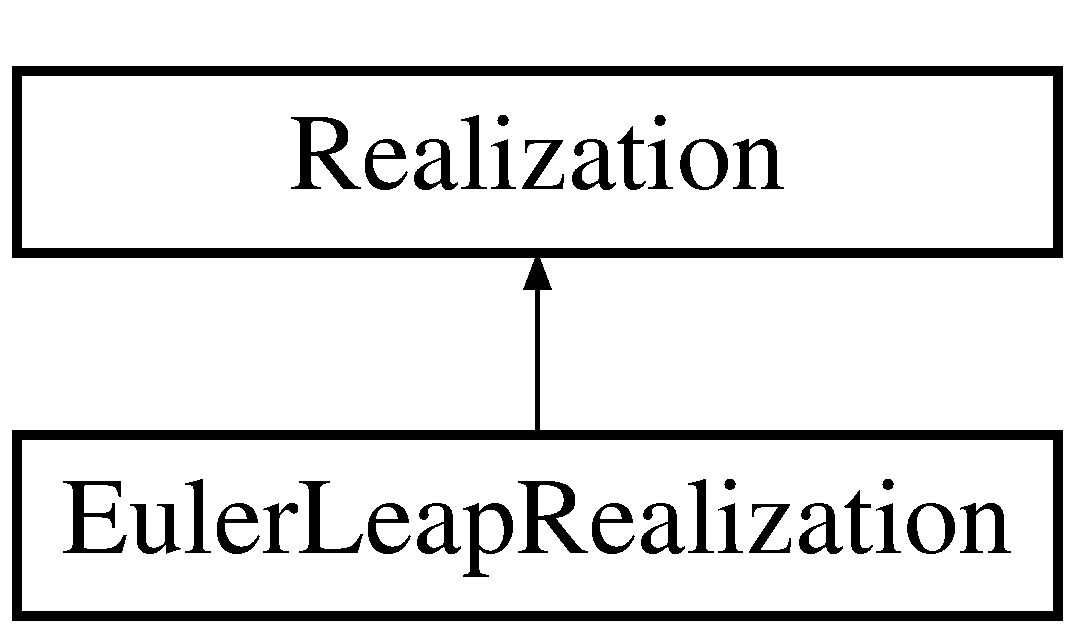
\includegraphics[height=2.000000cm]{class_euler_leap_realization}
\end{center}
\end{figure}
\subsection*{Public Member Functions}
\begin{DoxyCompactItemize}
\item 
\mbox{\Hypertarget{class_euler_leap_realization_ab72bfdc22d6101f2c10227b27a5121f1}\label{class_euler_leap_realization_ab72bfdc22d6101f2c10227b27a5121f1}} 
int {\bfseries step} ()
\end{DoxyCompactItemize}
\subsection*{Additional Inherited Members}


The documentation for this class was generated from the following file\+:\begin{DoxyCompactItemize}
\item 
/\+Users/\+Caleb/\+A\+P\+C524/stoched/src/realization.\+h\end{DoxyCompactItemize}

\hypertarget{class_event}{}\section{Event Class Reference}
\label{class_event}\index{Event@{Event}}


Class \hyperlink{class_event}{Event} holds a user-\/specified event, namely set of functions and associated rate.  




{\ttfamily \#include $<$event.\+h$>$}

\subsection*{Public Member Functions}
\begin{DoxyCompactItemize}
\item 
\hyperlink{class_event_a5a40dd4708297f7031e29b39e039ae10}{Event} ()
\begin{DoxyCompactList}\small\item\em Default constructor for \hyperlink{class_event}{Event}. \end{DoxyCompactList}\item 
\hyperlink{class_event_a7704ec01ce91e673885792054214b3d2}{$\sim$\+Event} ()
\begin{DoxyCompactList}\small\item\em Destructor of \hyperlink{class_event}{Event}. \end{DoxyCompactList}\item 
void \hyperlink{class_event_ad380e41418d2e34b651e052711fefe83}{add\+Function} (string function, string variables)
\begin{DoxyCompactList}\small\item\em Add a function parser to the function array. \end{DoxyCompactList}\item 
double \hyperlink{class_event_a2637844b7f9583caf0f808c898dc2246}{use\+Function} (int i\+Function, double $\ast$args)
\begin{DoxyCompactList}\small\item\em Evaluate function stored at specified spot in the function array. \end{DoxyCompactList}\item 
void \hyperlink{class_event_a993a01984496bc158be92b67422f8655}{set\+Rate} (string function, string variables)
\begin{DoxyCompactList}\small\item\em Set equation for rate\+Function. \end{DoxyCompactList}\item 
double \hyperlink{class_event_a2288e3b3fa19e076e04bba11b88d189a}{get\+Rate} (double $\ast$args)
\begin{DoxyCompactList}\small\item\em Return rate to user based on values of the state array. \end{DoxyCompactList}\item 
int \hyperlink{class_event_a1a0f2e2dc0b203f7be0f1d5b8810c6a2}{get\+Size} ()
\begin{DoxyCompactList}\small\item\em Return size of event, namely number of functions, to user. \end{DoxyCompactList}\item 
double \hyperlink{class_event_afb753b1954fd16e7ba92ae16157f70fd}{get\+Delta\+Var} (int i)
\begin{DoxyCompactList}\small\item\em Return how the ith variable is incremented when the ith equation is called. \end{DoxyCompactList}\item 
void \hyperlink{class_event_a980f39895f2afc1c2273d921d92aeac0}{set\+Delta\+Var} (int i, double val)
\begin{DoxyCompactList}\small\item\em set the amount that the ith function increments the ith variable. This is used by midpoint tau leaping \end{DoxyCompactList}\end{DoxyCompactItemize}
\subsection*{Public Attributes}
\begin{DoxyCompactItemize}
\item 
\mbox{\Hypertarget{class_event_acf8fc6215a0eeaa049e2aca9a347f4b0}\label{class_event_acf8fc6215a0eeaa049e2aca9a347f4b0}} 
string {\bfseries event\+Name}
\end{DoxyCompactItemize}
\subsection*{Private Attributes}
\begin{DoxyCompactItemize}
\item 
\mbox{\Hypertarget{class_event_a77f230a68021756fd1e2d35dcfa534f8}\label{class_event_a77f230a68021756fd1e2d35dcfa534f8}} 
Function\+Parser $\ast$$\ast$ \hyperlink{class_event_a77f230a68021756fd1e2d35dcfa534f8}{function\+Array\+\_\+}
\begin{DoxyCompactList}\small\item\em Array of function parsers. \end{DoxyCompactList}\item 
\mbox{\Hypertarget{class_event_a5a82a70465e39626ad62d1cfe3fc7617}\label{class_event_a5a82a70465e39626ad62d1cfe3fc7617}} 
Function\+Parser \hyperlink{class_event_a5a82a70465e39626ad62d1cfe3fc7617}{rate\+Function}
\begin{DoxyCompactList}\small\item\em Rate specified by an equation. \end{DoxyCompactList}\item 
\mbox{\Hypertarget{class_event_a59244ccd0e0f3654f07715bb3dd6423f}\label{class_event_a59244ccd0e0f3654f07715bb3dd6423f}} 
int \hyperlink{class_event_a59244ccd0e0f3654f07715bb3dd6423f}{eq\+\_\+count\+\_\+}
\begin{DoxyCompactList}\small\item\em Number of function parsers. \end{DoxyCompactList}\item 
\mbox{\Hypertarget{class_event_a869e25f5b77f85372eb0397ea01e25bf}\label{class_event_a869e25f5b77f85372eb0397ea01e25bf}} 
double $\ast$ \hyperlink{class_event_a869e25f5b77f85372eb0397ea01e25bf}{delta\+Var\+\_\+}
\begin{DoxyCompactList}\small\item\em how much each variable in the state changes when its corrsponding function is called. Only used by midpoint tau leaping to calculate approximate continuous time derivative. \end{DoxyCompactList}\end{DoxyCompactItemize}


\subsection{Detailed Description}
Class \hyperlink{class_event}{Event} holds a user-\/specified event, namely set of functions and associated rate. 

\subsection{Constructor \& Destructor Documentation}
\mbox{\Hypertarget{class_event_a5a40dd4708297f7031e29b39e039ae10}\label{class_event_a5a40dd4708297f7031e29b39e039ae10}} 
\index{Event@{Event}!Event@{Event}}
\index{Event@{Event}!Event@{Event}}
\subsubsection{\texorpdfstring{Event()}{Event()}}
{\footnotesize\ttfamily Event\+::\+Event (\begin{DoxyParamCaption}{ }\end{DoxyParamCaption})}



Default constructor for \hyperlink{class_event}{Event}. 


\begin{DoxyParams}{Parameters}
{\em eq\+\_\+count} & is the size of the function array \\
\hline
{\em function\+Array} & contains all user-\/specified Function\+Parsers that govern event \\
\hline
\end{DoxyParams}
\begin{DoxyReturn}{Returns}
nothing 
\end{DoxyReturn}
\mbox{\Hypertarget{class_event_a7704ec01ce91e673885792054214b3d2}\label{class_event_a7704ec01ce91e673885792054214b3d2}} 
\index{Event@{Event}!````~Event@{$\sim$\+Event}}
\index{````~Event@{$\sim$\+Event}!Event@{Event}}
\subsubsection{\texorpdfstring{$\sim$\+Event()}{~Event()}}
{\footnotesize\ttfamily Event\+::$\sim$\+Event (\begin{DoxyParamCaption}{ }\end{DoxyParamCaption})}



Destructor of \hyperlink{class_event}{Event}. 

\begin{DoxyReturn}{Returns}
nothing 
\end{DoxyReturn}


\subsection{Member Function Documentation}
\mbox{\Hypertarget{class_event_ad380e41418d2e34b651e052711fefe83}\label{class_event_ad380e41418d2e34b651e052711fefe83}} 
\index{Event@{Event}!add\+Function@{add\+Function}}
\index{add\+Function@{add\+Function}!Event@{Event}}
\subsubsection{\texorpdfstring{add\+Function()}{addFunction()}}
{\footnotesize\ttfamily void Event\+::add\+Function (\begin{DoxyParamCaption}\item[{string}]{function,  }\item[{string}]{variables }\end{DoxyParamCaption})}



Add a function parser to the function array. 


\begin{DoxyParams}{Parameters}
{\em function} & is a string used to generate a Function\+Parser object \\
\hline
{\em variables} & is a string used to generate a Function\+Parser object \\
\hline
\end{DoxyParams}
\begin{DoxyReturn}{Returns}
void 
\end{DoxyReturn}
\mbox{\Hypertarget{class_event_afb753b1954fd16e7ba92ae16157f70fd}\label{class_event_afb753b1954fd16e7ba92ae16157f70fd}} 
\index{Event@{Event}!get\+Delta\+Var@{get\+Delta\+Var}}
\index{get\+Delta\+Var@{get\+Delta\+Var}!Event@{Event}}
\subsubsection{\texorpdfstring{get\+Delta\+Var()}{getDeltaVar()}}
{\footnotesize\ttfamily double Event\+::get\+Delta\+Var (\begin{DoxyParamCaption}\item[{int}]{i }\end{DoxyParamCaption})}



Return how the ith variable is incremented when the ith equation is called. 


\begin{DoxyParams}{Parameters}
{\em i} & is an int specifying of which variable to find the delta. 0 is the first variable \\
\hline
\end{DoxyParams}
\begin{DoxyReturn}{Returns}
change in value of i when its corresponding equation is called, as a double 
\end{DoxyReturn}
\mbox{\Hypertarget{class_event_a2288e3b3fa19e076e04bba11b88d189a}\label{class_event_a2288e3b3fa19e076e04bba11b88d189a}} 
\index{Event@{Event}!get\+Rate@{get\+Rate}}
\index{get\+Rate@{get\+Rate}!Event@{Event}}
\subsubsection{\texorpdfstring{get\+Rate()}{getRate()}}
{\footnotesize\ttfamily double Event\+::get\+Rate (\begin{DoxyParamCaption}\item[{double $\ast$}]{state\+Array }\end{DoxyParamCaption})}



Return rate to user based on values of the state array. 


\begin{DoxyParams}{Parameters}
{\em state\+Array} & is a double array specifying variable values of function \\
\hline
\end{DoxyParams}
\begin{DoxyReturn}{Returns}
evaluated rate\+Function as a double 
\end{DoxyReturn}
\mbox{\Hypertarget{class_event_a1a0f2e2dc0b203f7be0f1d5b8810c6a2}\label{class_event_a1a0f2e2dc0b203f7be0f1d5b8810c6a2}} 
\index{Event@{Event}!get\+Size@{get\+Size}}
\index{get\+Size@{get\+Size}!Event@{Event}}
\subsubsection{\texorpdfstring{get\+Size()}{getSize()}}
{\footnotesize\ttfamily int Event\+::get\+Size (\begin{DoxyParamCaption}{ }\end{DoxyParamCaption})}



Return size of event, namely number of functions, to user. 

\begin{DoxyReturn}{Returns}
size of event, namely number of functions, as an int 
\end{DoxyReturn}
\mbox{\Hypertarget{class_event_a980f39895f2afc1c2273d921d92aeac0}\label{class_event_a980f39895f2afc1c2273d921d92aeac0}} 
\index{Event@{Event}!set\+Delta\+Var@{set\+Delta\+Var}}
\index{set\+Delta\+Var@{set\+Delta\+Var}!Event@{Event}}
\subsubsection{\texorpdfstring{set\+Delta\+Var()}{setDeltaVar()}}
{\footnotesize\ttfamily void Event\+::set\+Delta\+Var (\begin{DoxyParamCaption}\item[{int}]{i,  }\item[{double}]{val }\end{DoxyParamCaption})}



set the amount that the ith function increments the ith variable. This is used by midpoint tau leaping 


\begin{DoxyParams}{Parameters}
{\em i} & is an int specifying of which variable to set. 0 is the first variable \\
\hline
\end{DoxyParams}
\begin{DoxyReturn}{Returns}
void 
\end{DoxyReturn}
\mbox{\Hypertarget{class_event_a993a01984496bc158be92b67422f8655}\label{class_event_a993a01984496bc158be92b67422f8655}} 
\index{Event@{Event}!set\+Rate@{set\+Rate}}
\index{set\+Rate@{set\+Rate}!Event@{Event}}
\subsubsection{\texorpdfstring{set\+Rate()}{setRate()}}
{\footnotesize\ttfamily void Event\+::set\+Rate (\begin{DoxyParamCaption}\item[{string}]{function,  }\item[{string}]{variables }\end{DoxyParamCaption})}



Set equation for rate\+Function. 


\begin{DoxyParams}{Parameters}
{\em function} & is a string used for parsing rate\+Function \\
\hline
{\em variables} & is a string used for parsing rate\+Function \\
\hline
\end{DoxyParams}
\begin{DoxyReturn}{Returns}
void 
\end{DoxyReturn}
\mbox{\Hypertarget{class_event_a2637844b7f9583caf0f808c898dc2246}\label{class_event_a2637844b7f9583caf0f808c898dc2246}} 
\index{Event@{Event}!use\+Function@{use\+Function}}
\index{use\+Function@{use\+Function}!Event@{Event}}
\subsubsection{\texorpdfstring{use\+Function()}{useFunction()}}
{\footnotesize\ttfamily double Event\+::use\+Function (\begin{DoxyParamCaption}\item[{int}]{i\+Function,  }\item[{double $\ast$}]{state\+Array }\end{DoxyParamCaption})}



Evaluate function stored at specified spot in the function array. 


\begin{DoxyParams}{Parameters}
{\em i\+Function} & is an int that indexes function array \\
\hline
{\em state\+Array} & is a double array specifying variable values of function \\
\hline
\end{DoxyParams}
\begin{DoxyReturn}{Returns}
evaluated function\+Parser as a double 
\end{DoxyReturn}


The documentation for this class was generated from the following files\+:\begin{DoxyCompactItemize}
\item 
/\+Users/dylan/stoched/src/\hyperlink{event_8h}{event.\+h}\item 
/\+Users/dylan/stoched/src/\hyperlink{event_8cc}{event.\+cc}\end{DoxyCompactItemize}

\hypertarget{class_exact_realization}{}\section{Exact\+Realization Class Reference}
\label{class_exact_realization}\index{Exact\+Realization@{Exact\+Realization}}


Class \hyperlink{class_exact_realization}{Exact\+Realization} implements \hyperlink{class_realization}{Realization} \hyperlink{class_exact_realization_a3dfa40f473f2cfce2263f4d304af3828}{step()} function using exact calculation.  




{\ttfamily \#include $<$realization.\+h$>$}

Inheritance diagram for Exact\+Realization\+:\begin{figure}[H]
\begin{center}
\leavevmode
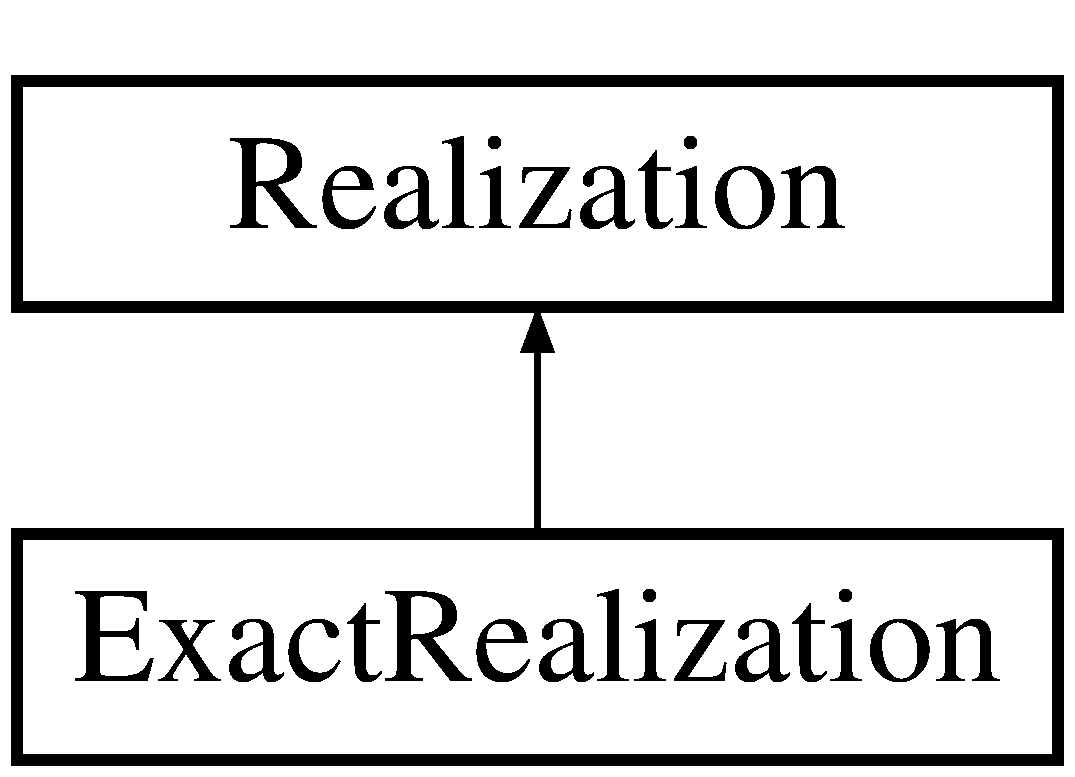
\includegraphics[height=2.000000cm]{class_exact_realization}
\end{center}
\end{figure}
\subsection*{Public Member Functions}
\begin{DoxyCompactItemize}
\item 
\mbox{\Hypertarget{class_exact_realization_a3dfa40f473f2cfce2263f4d304af3828}\label{class_exact_realization_a3dfa40f473f2cfce2263f4d304af3828}} 
int \hyperlink{class_exact_realization_a3dfa40f473f2cfce2263f4d304af3828}{step} ()
\begin{DoxyCompactList}\small\item\em takes one simulation step according to the chosen algorithm \end{DoxyCompactList}\end{DoxyCompactItemize}
\subsection*{Additional Inherited Members}


\subsection{Detailed Description}
Class \hyperlink{class_exact_realization}{Exact\+Realization} implements \hyperlink{class_realization}{Realization} \hyperlink{class_exact_realization_a3dfa40f473f2cfce2263f4d304af3828}{step()} function using exact calculation. 

The documentation for this class was generated from the following file\+:\begin{DoxyCompactItemize}
\item 
/\+Users/\+Caleb/\+A\+P\+C524/stoched/src/\hyperlink{realization_8h}{realization.\+h}\end{DoxyCompactItemize}

\hypertarget{class_midpoint_leap_realization}{}\section{Midpoint\+Leap\+Realization Class Reference}
\label{class_midpoint_leap_realization}\index{Midpoint\+Leap\+Realization@{Midpoint\+Leap\+Realization}}


Class \hyperlink{class_midpoint_leap_realization}{Midpoint\+Leap\+Realization} implements \hyperlink{class_realization}{Realization} \hyperlink{class_midpoint_leap_realization_a6c3e52150f488b7daccc2d0caa0cb378}{step()} function using Midpoint Leap method.  




{\ttfamily \#include $<$realization.\+h$>$}

Inheritance diagram for Midpoint\+Leap\+Realization\+:\begin{figure}[H]
\begin{center}
\leavevmode
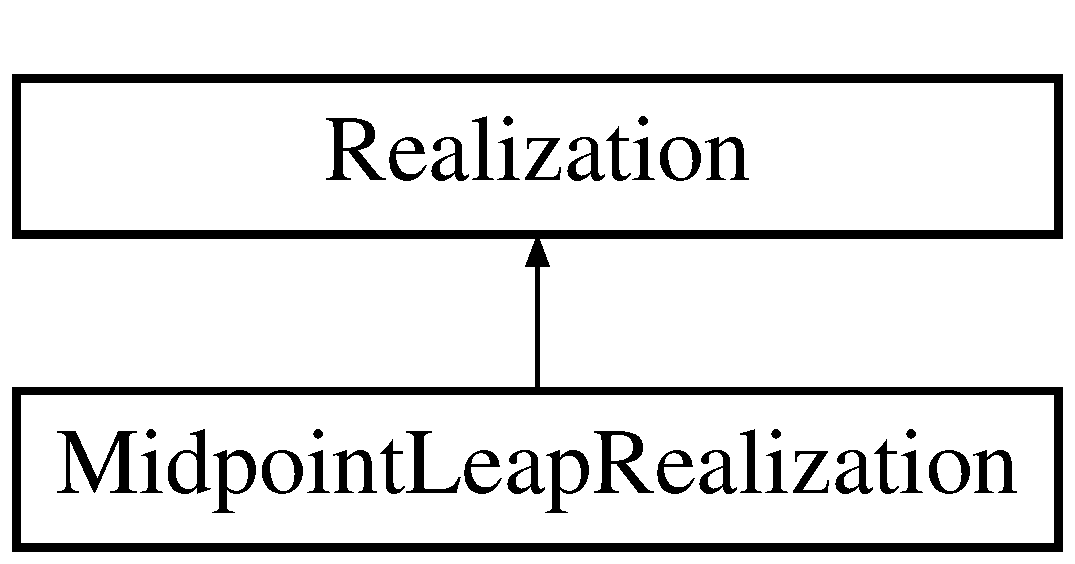
\includegraphics[height=2.000000cm]{class_midpoint_leap_realization}
\end{center}
\end{figure}
\subsection*{Public Member Functions}
\begin{DoxyCompactItemize}
\item 
\mbox{\Hypertarget{class_midpoint_leap_realization_a6c3e52150f488b7daccc2d0caa0cb378}\label{class_midpoint_leap_realization_a6c3e52150f488b7daccc2d0caa0cb378}} 
int \hyperlink{class_midpoint_leap_realization_a6c3e52150f488b7daccc2d0caa0cb378}{step} ()
\begin{DoxyCompactList}\small\item\em takes one simulation step according to the chosen algorithm \end{DoxyCompactList}\end{DoxyCompactItemize}
\subsection*{Additional Inherited Members}


\subsection{Detailed Description}
Class \hyperlink{class_midpoint_leap_realization}{Midpoint\+Leap\+Realization} implements \hyperlink{class_realization}{Realization} \hyperlink{class_midpoint_leap_realization_a6c3e52150f488b7daccc2d0caa0cb378}{step()} function using Midpoint Leap method. 

The documentation for this class was generated from the following file\+:\begin{DoxyCompactItemize}
\item 
/\+Users/\+Caleb/\+A\+P\+C524/stoched/src/\hyperlink{realization_8h}{realization.\+h}\end{DoxyCompactItemize}

\hypertarget{class_model}{}\section{Model Class Reference}
\label{class_model}\index{Model@{Model}}


Class M\+O\+D\+EL, which holds user-\/specified models of stochastic systems from which realizations are to be simulated. A model may have variable parameters; each complete set will be stored in an object of class \hyperlink{class_paramset}{Paramset}.  




{\ttfamily \#include $<$model.\+h$>$}

\subsection*{Public Member Functions}
\begin{DoxyCompactItemize}
\item 
\hyperlink{class_model_ae3b375de5f6df4faf74a95d64748e048}{Model} ()
\begin{DoxyCompactList}\small\item\em Default constructor for \hyperlink{class_model}{Model}. \end{DoxyCompactList}\item 
\hyperlink{class_model_ad6ebd2062a0b823db841a0b88baac4c0}{$\sim$\+Model} ()
\begin{DoxyCompactList}\small\item\em Destructor of \hyperlink{class_model}{Model}. \end{DoxyCompactList}\item 
void \hyperlink{class_model_a4743b4f267eeb1a60e21cc2995e1efcd}{add\+Vars} (string vars)
\begin{DoxyCompactList}\small\item\em Add variable list to a \hyperlink{class_model}{Model}. \end{DoxyCompactList}\item 
void \hyperlink{class_model_ab6f784e4ff8cdf3ee5e010ef4dd8d597}{add\+Event} (string function\+Rate)
\begin{DoxyCompactList}\small\item\em Add \hyperlink{class_event}{Event} to \hyperlink{class_model}{Model}\textquotesingle{}s list of Events. \end{DoxyCompactList}\item 
void \hyperlink{class_model_a78d9b07bd5e819215c9aeefabb4cede7}{add\+Event\+Fct} (int i\+Event, string function)
\begin{DoxyCompactList}\small\item\em Add \hyperlink{class_event}{Event} function to specified \hyperlink{class_event}{Event} in \hyperlink{class_model}{Model}. \end{DoxyCompactList}\item 
double \hyperlink{class_model_a774d9fb034f8704a75d7b3568a87a3bc}{use\+Event\+Fct} (int i\+Event, int i\+Function, double $\ast$state\+Array)
\begin{DoxyCompactList}\small\item\em Evaluate given function in specified \hyperlink{class_event}{Event}. \end{DoxyCompactList}\item 
double \hyperlink{class_model_a2909caddddccca90faaae708e68226ad}{get\+Event\+Rate} (int i\+Event, double $\ast$state\+Array)
\begin{DoxyCompactList}\small\item\em Evaluate rate function for a specified \hyperlink{class_event}{Event}. \end{DoxyCompactList}\item 
void \hyperlink{class_model_ad9e7a181a31a2a9fab052d11b1984afd}{update\+State} (int i\+Event, double $\ast$state\+Array)
\begin{DoxyCompactList}\small\item\em Update state array by evaluating all functions of a given \hyperlink{class_event}{Event}. \end{DoxyCompactList}\item 
void \hyperlink{class_model_a3f2fd71261c87162718864d7efc67f2f}{update\+Rates} (double $\ast$state\+Array, double $\ast$rate\+Array)
\begin{DoxyCompactList}\small\item\em Update rate for all Events in \hyperlink{class_model}{Model}\textquotesingle{}s \hyperlink{class_event}{Event} list. \end{DoxyCompactList}\end{DoxyCompactItemize}


\subsection{Detailed Description}
Class M\+O\+D\+EL, which holds user-\/specified models of stochastic systems from which realizations are to be simulated. A model may have variable parameters; each complete set will be stored in an object of class \hyperlink{class_paramset}{Paramset}. 

\subsection{Constructor \& Destructor Documentation}
\mbox{\Hypertarget{class_model_ae3b375de5f6df4faf74a95d64748e048}\label{class_model_ae3b375de5f6df4faf74a95d64748e048}} 
\index{Model@{Model}!Model@{Model}}
\index{Model@{Model}!Model@{Model}}
\subsubsection{\texorpdfstring{Model()}{Model()}}
{\footnotesize\ttfamily Model\+::\+Model (\begin{DoxyParamCaption}{ }\end{DoxyParamCaption})}



Default constructor for \hyperlink{class_model}{Model}. 


\begin{DoxyParams}{Parameters}
{\em none} & \\
\hline
\end{DoxyParams}
\begin{DoxyReturn}{Returns}
nothing 
\end{DoxyReturn}
\mbox{\Hypertarget{class_model_ad6ebd2062a0b823db841a0b88baac4c0}\label{class_model_ad6ebd2062a0b823db841a0b88baac4c0}} 
\index{Model@{Model}!````~Model@{$\sim$\+Model}}
\index{````~Model@{$\sim$\+Model}!Model@{Model}}
\subsubsection{\texorpdfstring{$\sim$\+Model()}{~Model()}}
{\footnotesize\ttfamily Model\+::$\sim$\+Model (\begin{DoxyParamCaption}{ }\end{DoxyParamCaption})}



Destructor of \hyperlink{class_model}{Model}. 


\begin{DoxyParams}{Parameters}
{\em none} & \\
\hline
\end{DoxyParams}
\begin{DoxyReturn}{Returns}
nothing 
\end{DoxyReturn}


\subsection{Member Function Documentation}
\mbox{\Hypertarget{class_model_ab6f784e4ff8cdf3ee5e010ef4dd8d597}\label{class_model_ab6f784e4ff8cdf3ee5e010ef4dd8d597}} 
\index{Model@{Model}!add\+Event@{add\+Event}}
\index{add\+Event@{add\+Event}!Model@{Model}}
\subsubsection{\texorpdfstring{add\+Event()}{addEvent()}}
{\footnotesize\ttfamily void Model\+::add\+Event (\begin{DoxyParamCaption}\item[{string}]{function\+Rate }\end{DoxyParamCaption})}



Add \hyperlink{class_event}{Event} to \hyperlink{class_model}{Model}\textquotesingle{}s list of Events. 


\begin{DoxyParams}{Parameters}
{\em function\+Rate} & is a string that defines an \hyperlink{class_event}{Event}\textquotesingle{}s rate \\
\hline
\end{DoxyParams}
\begin{DoxyReturn}{Returns}
void 
\end{DoxyReturn}
\mbox{\Hypertarget{class_model_a78d9b07bd5e819215c9aeefabb4cede7}\label{class_model_a78d9b07bd5e819215c9aeefabb4cede7}} 
\index{Model@{Model}!add\+Event\+Fct@{add\+Event\+Fct}}
\index{add\+Event\+Fct@{add\+Event\+Fct}!Model@{Model}}
\subsubsection{\texorpdfstring{add\+Event\+Fct()}{addEventFct()}}
{\footnotesize\ttfamily void Model\+::add\+Event\+Fct (\begin{DoxyParamCaption}\item[{int}]{i\+Event,  }\item[{string}]{function }\end{DoxyParamCaption})}



Add \hyperlink{class_event}{Event} function to specified \hyperlink{class_event}{Event} in \hyperlink{class_model}{Model}. 


\begin{DoxyParams}{Parameters}
{\em i\+Event} & is an int that indexes \hyperlink{class_event}{Event} list \\
\hline
{\em function} & is a string that specifies \hyperlink{class_event}{Event} function \\
\hline
\end{DoxyParams}
\begin{DoxyReturn}{Returns}
void 
\end{DoxyReturn}
\mbox{\Hypertarget{class_model_a4743b4f267eeb1a60e21cc2995e1efcd}\label{class_model_a4743b4f267eeb1a60e21cc2995e1efcd}} 
\index{Model@{Model}!add\+Vars@{add\+Vars}}
\index{add\+Vars@{add\+Vars}!Model@{Model}}
\subsubsection{\texorpdfstring{add\+Vars()}{addVars()}}
{\footnotesize\ttfamily void Model\+::add\+Vars (\begin{DoxyParamCaption}\item[{string}]{vars }\end{DoxyParamCaption})}



Add variable list to a \hyperlink{class_model}{Model}. 


\begin{DoxyParams}{Parameters}
{\em vars} & is a string used to set variables associate with a \hyperlink{class_model}{Model} \\
\hline
\end{DoxyParams}
\begin{DoxyReturn}{Returns}
void 
\end{DoxyReturn}
\mbox{\Hypertarget{class_model_a2909caddddccca90faaae708e68226ad}\label{class_model_a2909caddddccca90faaae708e68226ad}} 
\index{Model@{Model}!get\+Event\+Rate@{get\+Event\+Rate}}
\index{get\+Event\+Rate@{get\+Event\+Rate}!Model@{Model}}
\subsubsection{\texorpdfstring{get\+Event\+Rate()}{getEventRate()}}
{\footnotesize\ttfamily double Model\+::get\+Event\+Rate (\begin{DoxyParamCaption}\item[{int}]{i\+Event,  }\item[{double $\ast$}]{state\+Array }\end{DoxyParamCaption})}



Evaluate rate function for a specified \hyperlink{class_event}{Event}. 


\begin{DoxyParams}{Parameters}
{\em i\+Event} & is an int that indexes \hyperlink{class_event}{Event} list \\
\hline
{\em state\+Array} & is a double array specifiying variable values of a function \\
\hline
\end{DoxyParams}
\begin{DoxyReturn}{Returns}
evaluated rate function as a double 
\end{DoxyReturn}
\mbox{\Hypertarget{class_model_a3f2fd71261c87162718864d7efc67f2f}\label{class_model_a3f2fd71261c87162718864d7efc67f2f}} 
\index{Model@{Model}!update\+Rates@{update\+Rates}}
\index{update\+Rates@{update\+Rates}!Model@{Model}}
\subsubsection{\texorpdfstring{update\+Rates()}{updateRates()}}
{\footnotesize\ttfamily void Model\+::update\+Rates (\begin{DoxyParamCaption}\item[{double $\ast$}]{state\+Array,  }\item[{double $\ast$}]{rate\+Array }\end{DoxyParamCaption})}



Update rate for all Events in \hyperlink{class_model}{Model}\textquotesingle{}s \hyperlink{class_event}{Event} list. 


\begin{DoxyParams}{Parameters}
{\em state\+Array} & is a double array specifiying variable values of a function \\
\hline
{\em rate\+Array} & is a double array specifiying variable values of a rate function \\
\hline
\end{DoxyParams}
\begin{DoxyReturn}{Returns}
void 
\end{DoxyReturn}
\mbox{\Hypertarget{class_model_ad9e7a181a31a2a9fab052d11b1984afd}\label{class_model_ad9e7a181a31a2a9fab052d11b1984afd}} 
\index{Model@{Model}!update\+State@{update\+State}}
\index{update\+State@{update\+State}!Model@{Model}}
\subsubsection{\texorpdfstring{update\+State()}{updateState()}}
{\footnotesize\ttfamily void Model\+::update\+State (\begin{DoxyParamCaption}\item[{int}]{i\+Event,  }\item[{double $\ast$}]{state\+Array }\end{DoxyParamCaption})}



Update state array by evaluating all functions of a given \hyperlink{class_event}{Event}. 


\begin{DoxyParams}{Parameters}
{\em i\+Event} & is an int that indexes \hyperlink{class_event}{Event} list \\
\hline
{\em state\+Array} & is a double array specifiying variable values of a function \\
\hline
\end{DoxyParams}
\begin{DoxyReturn}{Returns}
void 
\end{DoxyReturn}
\mbox{\Hypertarget{class_model_a774d9fb034f8704a75d7b3568a87a3bc}\label{class_model_a774d9fb034f8704a75d7b3568a87a3bc}} 
\index{Model@{Model}!use\+Event\+Fct@{use\+Event\+Fct}}
\index{use\+Event\+Fct@{use\+Event\+Fct}!Model@{Model}}
\subsubsection{\texorpdfstring{use\+Event\+Fct()}{useEventFct()}}
{\footnotesize\ttfamily double Model\+::use\+Event\+Fct (\begin{DoxyParamCaption}\item[{int}]{i\+Event,  }\item[{int}]{i\+Function,  }\item[{double $\ast$}]{state\+Array }\end{DoxyParamCaption})}



Evaluate given function in specified \hyperlink{class_event}{Event}. 


\begin{DoxyParams}{Parameters}
{\em i\+Event} & is an int that indexes \hyperlink{class_event}{Event} list \\
\hline
{\em i\+Function} & is an int that indexes an \hyperlink{class_event}{Event}\textquotesingle{}s Function list \\
\hline
{\em state\+Array} & is a double array specifiying variable values of a function \\
\hline
\end{DoxyParams}
\begin{DoxyReturn}{Returns}
evaluated function as a double 
\end{DoxyReturn}


The documentation for this class was generated from the following files\+:\begin{DoxyCompactItemize}
\item 
/\+Users/\+Caleb/\+A\+P\+C524/stoched/src/model.\+h\item 
/\+Users/\+Caleb/\+A\+P\+C524/stoched/src/\hyperlink{model_8cc}{model.\+cc}\end{DoxyCompactItemize}

\hypertarget{class_paramset}{}\section{Paramset Class Reference}
\label{class_paramset}\index{Paramset@{Paramset}}


Class \hyperlink{class_paramset}{Paramset} holds a particular set of pameters for user requested simulation run(s)  




{\ttfamily \#include $<$paramset.\+h$>$}

\subsection*{Public Member Functions}
\begin{DoxyCompactItemize}
\item 
\hyperlink{class_paramset_aa62d7992b29e74983af7d6026b7111c0}{Paramset} (int \hyperlink{class_paramset_a67376577973f825ba60fc7c319ccc906}{method}, int \hyperlink{class_paramset_aee56c5dcf7d40836397965cdcf392343}{n\+\_\+vars}, double $\ast$\hyperlink{class_paramset_aae7232620d4a9c0bbf30b12c37610c1e}{initial\+\_\+values}, double \hyperlink{class_paramset_a7d82a76c08567e5072aa1b125708c7d8}{t\+\_\+initial}, double \hyperlink{class_paramset_ac88cde461d8dbbd8a7d2636fc45f7119}{t\+\_\+final}, double \hyperlink{class_paramset_a0554913cf803a67bc59ffdee154abc24}{timestep\+\_\+size}, int \hyperlink{class_paramset_a50c0325e75983b66d0825406ec7873ac}{n\+\_\+realizations}, int \hyperlink{class_paramset_afeb86c327cd6966707996019609e6ed1}{max\+\_\+iter}, int \hyperlink{class_paramset_ab8a5866bb87cc2d78a69c47bacaeb06e}{seed})
\begin{DoxyCompactList}\small\item\em Default constructor for \hyperlink{class_paramset}{Paramset}. \end{DoxyCompactList}\item 
\hyperlink{class_paramset_af05c1383de964a28d93e0630d2f4670e}{$\sim$\+Paramset} ()
\begin{DoxyCompactList}\small\item\em Destructor for \hyperlink{class_paramset}{Paramset}. \end{DoxyCompactList}\end{DoxyCompactItemize}
\subsection*{Public Attributes}
\begin{DoxyCompactItemize}
\item 
\mbox{\Hypertarget{class_paramset_a67376577973f825ba60fc7c319ccc906}\label{class_paramset_a67376577973f825ba60fc7c319ccc906}} 
const int \hyperlink{class_paramset_a67376577973f825ba60fc7c319ccc906}{method}
\begin{DoxyCompactList}\small\item\em which algorithm to use for simulation \end{DoxyCompactList}\item 
\mbox{\Hypertarget{class_paramset_aee56c5dcf7d40836397965cdcf392343}\label{class_paramset_aee56c5dcf7d40836397965cdcf392343}} 
const int \hyperlink{class_paramset_aee56c5dcf7d40836397965cdcf392343}{n\+\_\+vars}
\begin{DoxyCompactList}\small\item\em number of initial values/variables \end{DoxyCompactList}\item 
\mbox{\Hypertarget{class_paramset_aae7232620d4a9c0bbf30b12c37610c1e}\label{class_paramset_aae7232620d4a9c0bbf30b12c37610c1e}} 
const double $\ast$ \hyperlink{class_paramset_aae7232620d4a9c0bbf30b12c37610c1e}{initial\+\_\+values}
\begin{DoxyCompactList}\small\item\em initial values for variables \end{DoxyCompactList}\item 
\mbox{\Hypertarget{class_paramset_a7d82a76c08567e5072aa1b125708c7d8}\label{class_paramset_a7d82a76c08567e5072aa1b125708c7d8}} 
const double \hyperlink{class_paramset_a7d82a76c08567e5072aa1b125708c7d8}{t\+\_\+initial}
\begin{DoxyCompactList}\small\item\em initial time for simulation \end{DoxyCompactList}\item 
\mbox{\Hypertarget{class_paramset_ac88cde461d8dbbd8a7d2636fc45f7119}\label{class_paramset_ac88cde461d8dbbd8a7d2636fc45f7119}} 
const double \hyperlink{class_paramset_ac88cde461d8dbbd8a7d2636fc45f7119}{t\+\_\+final}
\begin{DoxyCompactList}\small\item\em final time for simulation \end{DoxyCompactList}\item 
\mbox{\Hypertarget{class_paramset_a0554913cf803a67bc59ffdee154abc24}\label{class_paramset_a0554913cf803a67bc59ffdee154abc24}} 
const double \hyperlink{class_paramset_a0554913cf803a67bc59ffdee154abc24}{timestep\+\_\+size}
\begin{DoxyCompactList}\small\item\em size of timestep for approximate \end{DoxyCompactList}\item 
\mbox{\Hypertarget{class_paramset_a50c0325e75983b66d0825406ec7873ac}\label{class_paramset_a50c0325e75983b66d0825406ec7873ac}} 
int \hyperlink{class_paramset_a50c0325e75983b66d0825406ec7873ac}{n\+\_\+realizations}
\begin{DoxyCompactList}\small\item\em number of realizations to simulate \end{DoxyCompactList}\item 
\mbox{\Hypertarget{class_paramset_afeb86c327cd6966707996019609e6ed1}\label{class_paramset_afeb86c327cd6966707996019609e6ed1}} 
int \hyperlink{class_paramset_afeb86c327cd6966707996019609e6ed1}{max\+\_\+iter}
\begin{DoxyCompactList}\small\item\em max number of iterations to simulate \end{DoxyCompactList}\item 
\mbox{\Hypertarget{class_paramset_ab8a5866bb87cc2d78a69c47bacaeb06e}\label{class_paramset_ab8a5866bb87cc2d78a69c47bacaeb06e}} 
int \hyperlink{class_paramset_ab8a5866bb87cc2d78a69c47bacaeb06e}{seed}
\begin{DoxyCompactList}\small\item\em seed for the random number generator \end{DoxyCompactList}\end{DoxyCompactItemize}


\subsection{Detailed Description}
Class \hyperlink{class_paramset}{Paramset} holds a particular set of pameters for user requested simulation run(s) 

\subsection{Constructor \& Destructor Documentation}
\mbox{\Hypertarget{class_paramset_aa62d7992b29e74983af7d6026b7111c0}\label{class_paramset_aa62d7992b29e74983af7d6026b7111c0}} 
\index{Paramset@{Paramset}!Paramset@{Paramset}}
\index{Paramset@{Paramset}!Paramset@{Paramset}}
\subsubsection{\texorpdfstring{Paramset()}{Paramset()}}
{\footnotesize\ttfamily Paramset\+::\+Paramset (\begin{DoxyParamCaption}\item[{int}]{method,  }\item[{int}]{n\+\_\+vars,  }\item[{double $\ast$}]{initial\+\_\+values,  }\item[{double}]{t\+\_\+initial,  }\item[{double}]{t\+\_\+final,  }\item[{double}]{timestep\+\_\+size,  }\item[{int}]{n\+\_\+realizations,  }\item[{int}]{max\+\_\+iter,  }\item[{int}]{seed }\end{DoxyParamCaption})}



Default constructor for \hyperlink{class_paramset}{Paramset}. 


\begin{DoxyParams}{Parameters}
{\em method} & is an int that specifies algorithm to use for simulation \\
\hline
{\em n\+\_\+vars} & is an int that specifies number of variables \\
\hline
{\em initial\+\_\+values} & is a double array that sets initial values for variables \\
\hline
{\em t\+\_\+initial} & is a double that sets initial time for simulation \\
\hline
{\em t\+\_\+final} & is a double that sets initial time for simulation \\
\hline
{\em timestep\+\_\+size} & is a double representing the size of the timestep for approximate methods \\
\hline
{\em n\+\_\+realizations} & is an int representing number of realizations to simulate \\
\hline
{\em max\+\_\+iter} & is an int and is the maximum number of iterations to simulate \\
\hline
\end{DoxyParams}
\mbox{\Hypertarget{class_paramset_af05c1383de964a28d93e0630d2f4670e}\label{class_paramset_af05c1383de964a28d93e0630d2f4670e}} 
\index{Paramset@{Paramset}!````~Paramset@{$\sim$\+Paramset}}
\index{````~Paramset@{$\sim$\+Paramset}!Paramset@{Paramset}}
\subsubsection{\texorpdfstring{$\sim$\+Paramset()}{~Paramset()}}
{\footnotesize\ttfamily Paramset\+::$\sim$\+Paramset (\begin{DoxyParamCaption}{ }\end{DoxyParamCaption})}



Destructor for \hyperlink{class_paramset}{Paramset}. 

\begin{DoxyReturn}{Returns}
nothing 
\end{DoxyReturn}


The documentation for this class was generated from the following files\+:\begin{DoxyCompactItemize}
\item 
/\+Users/\+Caleb/\+A\+P\+C524/stoched/src/\hyperlink{paramset_8h}{paramset.\+h}\item 
/\+Users/\+Caleb/\+A\+P\+C524/stoched/src/\hyperlink{paramset_8cc}{paramset.\+cc}\end{DoxyCompactItemize}

\hypertarget{class_realization}{}\section{Realization Class Reference}
\label{class_realization}\index{Realization@{Realization}}


Class \hyperlink{class_realization}{Realization} holds realizations of a \hyperlink{class_model}{Model} (state array, propensities, waiting times, etc.)  




{\ttfamily \#include $<$realization.\+h$>$}

Inheritance diagram for Realization\+:\begin{figure}[H]
\begin{center}
\leavevmode
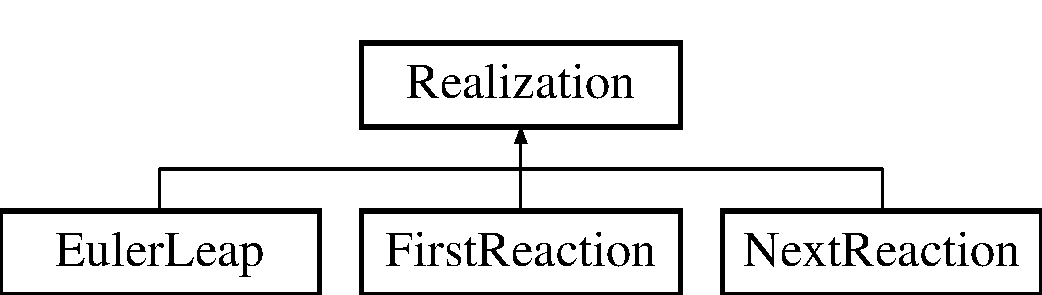
\includegraphics[height=2.000000cm]{class_realization}
\end{center}
\end{figure}
\subsection*{Public Member Functions}
\begin{DoxyCompactItemize}
\item 
\hyperlink{class_realization_af4cfb6f2221bef9ba5ad09564796677f}{Realization} (\hyperlink{class_model}{Model} $\ast$\hyperlink{class_realization_a47ec1d062b8caee874b08c1a17d6aeeb}{the\+\_\+model}, const \hyperlink{class_paramset}{Paramset} \&\hyperlink{class_realization_a119bb29de88929bc51bc1b329473a94b}{the\+\_\+paramset}, \hyperlink{classrng}{rng} $\ast$\hyperlink{class_realization_ac8d358d929afae90cf5790675b6744f9}{the\+\_\+rng}, int \hyperlink{class_realization_ad9951a0829e68e12fcb3817735bb5097}{n\+\_\+vars}, int \hyperlink{class_realization_afb711282bef806fc0020f91252d1df2c}{n\+\_\+events})
\begin{DoxyCompactList}\small\item\em Default constructor for \hyperlink{class_realization}{Realization}. \end{DoxyCompactList}\item 
virtual \hyperlink{class_realization_a040c39b39c5057c668bd264b4329f2b4}{$\sim$\+Realization} ()
\begin{DoxyCompactList}\small\item\em Destructor of \hyperlink{class_realization}{Realization}. \end{DoxyCompactList}\item 
int \hyperlink{class_realization_a4e21bc7355e33c17d1401736b3c62413}{simulate} (std\+::ofstream \&myfile)
\begin{DoxyCompactList}\small\item\em Simulates the realization from t\+\_\+inital to t\+\_\+final. \end{DoxyCompactList}\item 
\mbox{\Hypertarget{class_realization_a9949217117927b149850288f3b74c9ef}\label{class_realization_a9949217117927b149850288f3b74c9ef}} 
virtual int \hyperlink{class_realization_a9949217117927b149850288f3b74c9ef}{step} ()=0
\begin{DoxyCompactList}\small\item\em takes one simulation step according to the chosen algorithm \end{DoxyCompactList}\item 
bool \hyperlink{class_realization_a48953442ebf235cd1e02731c7419f65f}{rates\+\_\+are\+\_\+zero} ()
\begin{DoxyCompactList}\small\item\em checks whether all rates are zero \end{DoxyCompactList}\item 
int \hyperlink{class_realization_ab7ef90279eef4bf11261084f541c7bb0}{output\+\_\+state} (std\+::ofstream \&myfile)
\begin{DoxyCompactList}\small\item\em Prints the current state of the simulation. \end{DoxyCompactList}\item 
virtual int \hyperlink{class_realization_a391a89af7574a9053f53f8a299c2cc70}{set\+\_\+to\+\_\+initial\+\_\+state} ()
\begin{DoxyCompactList}\small\item\em Sets state\+\_\+array and state\+\_\+time to their user-\/specified initial values. \end{DoxyCompactList}\end{DoxyCompactItemize}
\subsection*{Public Attributes}
\begin{DoxyCompactItemize}
\item 
\mbox{\Hypertarget{class_realization_a47ec1d062b8caee874b08c1a17d6aeeb}\label{class_realization_a47ec1d062b8caee874b08c1a17d6aeeb}} 
\hyperlink{class_model}{Model} $\ast$ \hyperlink{class_realization_a47ec1d062b8caee874b08c1a17d6aeeb}{the\+\_\+model}
\begin{DoxyCompactList}\small\item\em the\+\_\+model is a \hyperlink{class_model}{Model} instance \end{DoxyCompactList}\item 
\mbox{\Hypertarget{class_realization_a119bb29de88929bc51bc1b329473a94b}\label{class_realization_a119bb29de88929bc51bc1b329473a94b}} 
const \hyperlink{class_paramset}{Paramset} \hyperlink{class_realization_a119bb29de88929bc51bc1b329473a94b}{the\+\_\+paramset}
\begin{DoxyCompactList}\small\item\em the\+\_\+paramset is a \hyperlink{class_paramset}{Paramset} instance \end{DoxyCompactList}\item 
\mbox{\Hypertarget{class_realization_ac8d358d929afae90cf5790675b6744f9}\label{class_realization_ac8d358d929afae90cf5790675b6744f9}} 
\hyperlink{classrng}{rng} $\ast$ \hyperlink{class_realization_ac8d358d929afae90cf5790675b6744f9}{the\+\_\+rng}
\begin{DoxyCompactList}\small\item\em the\+\_\+rng is an random number generator \end{DoxyCompactList}\item 
\mbox{\Hypertarget{class_realization_ad9951a0829e68e12fcb3817735bb5097}\label{class_realization_ad9951a0829e68e12fcb3817735bb5097}} 
const int \hyperlink{class_realization_ad9951a0829e68e12fcb3817735bb5097}{n\+\_\+vars}
\begin{DoxyCompactList}\small\item\em n\+\_\+vars is an int specifying number of variables \end{DoxyCompactList}\item 
\mbox{\Hypertarget{class_realization_afb711282bef806fc0020f91252d1df2c}\label{class_realization_afb711282bef806fc0020f91252d1df2c}} 
const int \hyperlink{class_realization_afb711282bef806fc0020f91252d1df2c}{n\+\_\+events}
\begin{DoxyCompactList}\small\item\em n\+\_\+events is an int specifying number of events \end{DoxyCompactList}\item 
\mbox{\Hypertarget{class_realization_a126f89978f0407873473222171333ee1}\label{class_realization_a126f89978f0407873473222171333ee1}} 
double $\ast$ \hyperlink{class_realization_a126f89978f0407873473222171333ee1}{state\+\_\+array}
\begin{DoxyCompactList}\small\item\em state\+\_\+array is a double array specifiying variable values of a function \end{DoxyCompactList}\item 
\mbox{\Hypertarget{class_realization_a9c52d8c6aa0ad99dbbec1e98302db7d8}\label{class_realization_a9c52d8c6aa0ad99dbbec1e98302db7d8}} 
double $\ast$ \hyperlink{class_realization_a9c52d8c6aa0ad99dbbec1e98302db7d8}{rates}
\begin{DoxyCompactList}\small\item\em rates is a double array specifying variable values of a rate function \end{DoxyCompactList}\item 
\mbox{\Hypertarget{class_realization_a7c4def45c4833072317517b71e723793}\label{class_realization_a7c4def45c4833072317517b71e723793}} 
double \hyperlink{class_realization_a7c4def45c4833072317517b71e723793}{state\+\_\+time}
\begin{DoxyCompactList}\small\item\em state\+\_\+time is a double that tracks state progress \end{DoxyCompactList}\end{DoxyCompactItemize}


\subsection{Detailed Description}
Class \hyperlink{class_realization}{Realization} holds realizations of a \hyperlink{class_model}{Model} (state array, propensities, waiting times, etc.) 

\subsection{Constructor \& Destructor Documentation}
\mbox{\Hypertarget{class_realization_af4cfb6f2221bef9ba5ad09564796677f}\label{class_realization_af4cfb6f2221bef9ba5ad09564796677f}} 
\index{Realization@{Realization}!Realization@{Realization}}
\index{Realization@{Realization}!Realization@{Realization}}
\subsubsection{\texorpdfstring{Realization()}{Realization()}}
{\footnotesize\ttfamily Realization\+::\+Realization (\begin{DoxyParamCaption}\item[{\hyperlink{class_model}{Model} $\ast$}]{the\+\_\+model,  }\item[{const \hyperlink{class_paramset}{Paramset} \&}]{the\+\_\+paramset,  }\item[{\hyperlink{classrng}{rng} $\ast$}]{the\+\_\+rng,  }\item[{int}]{n\+\_\+vars,  }\item[{int}]{n\+\_\+events }\end{DoxyParamCaption})}



Default constructor for \hyperlink{class_realization}{Realization}. 


\begin{DoxyParams}{Parameters}
{\em the\+\_\+model} & is a \hyperlink{class_model}{Model} object \\
\hline
{\em the\+\_\+paramset} & is a \hyperlink{class_paramset}{Paramset} object \\
\hline
{\em the\+\_\+rng} & is a random number generator \\
\hline
{\em n\+\_\+vars} & is an int specifying variable count \\
\hline
{\em n\+\_\+events} & is an int specifying event count\\
\hline
\end{DoxyParams}
\begin{DoxyReturn}{Returns}
nothing 
\end{DoxyReturn}
\mbox{\Hypertarget{class_realization_a040c39b39c5057c668bd264b4329f2b4}\label{class_realization_a040c39b39c5057c668bd264b4329f2b4}} 
\index{Realization@{Realization}!````~Realization@{$\sim$\+Realization}}
\index{````~Realization@{$\sim$\+Realization}!Realization@{Realization}}
\subsubsection{\texorpdfstring{$\sim$\+Realization()}{~Realization()}}
{\footnotesize\ttfamily Realization\+::$\sim$\+Realization (\begin{DoxyParamCaption}{ }\end{DoxyParamCaption})\hspace{0.3cm}{\ttfamily [virtual]}}



Destructor of \hyperlink{class_realization}{Realization}. 

\begin{DoxyReturn}{Returns}
nothing 
\end{DoxyReturn}


\subsection{Member Function Documentation}
\mbox{\Hypertarget{class_realization_ab7ef90279eef4bf11261084f541c7bb0}\label{class_realization_ab7ef90279eef4bf11261084f541c7bb0}} 
\index{Realization@{Realization}!output\+\_\+state@{output\+\_\+state}}
\index{output\+\_\+state@{output\+\_\+state}!Realization@{Realization}}
\subsubsection{\texorpdfstring{output\+\_\+state()}{output\_state()}}
{\footnotesize\ttfamily int Realization\+::output\+\_\+state (\begin{DoxyParamCaption}\item[{std\+::ofstream \&}]{myfile }\end{DoxyParamCaption})}



Prints the current state of the simulation. 

\begin{DoxyReturn}{Returns}
int 
\end{DoxyReturn}
\mbox{\Hypertarget{class_realization_a48953442ebf235cd1e02731c7419f65f}\label{class_realization_a48953442ebf235cd1e02731c7419f65f}} 
\index{Realization@{Realization}!rates\+\_\+are\+\_\+zero@{rates\+\_\+are\+\_\+zero}}
\index{rates\+\_\+are\+\_\+zero@{rates\+\_\+are\+\_\+zero}!Realization@{Realization}}
\subsubsection{\texorpdfstring{rates\+\_\+are\+\_\+zero()}{rates\_are\_zero()}}
{\footnotesize\ttfamily bool Realization\+::rates\+\_\+are\+\_\+zero (\begin{DoxyParamCaption}{ }\end{DoxyParamCaption})}



checks whether all rates are zero 

\begin{DoxyReturn}{Returns}
bool 
\end{DoxyReturn}
\mbox{\Hypertarget{class_realization_a391a89af7574a9053f53f8a299c2cc70}\label{class_realization_a391a89af7574a9053f53f8a299c2cc70}} 
\index{Realization@{Realization}!set\+\_\+to\+\_\+initial\+\_\+state@{set\+\_\+to\+\_\+initial\+\_\+state}}
\index{set\+\_\+to\+\_\+initial\+\_\+state@{set\+\_\+to\+\_\+initial\+\_\+state}!Realization@{Realization}}
\subsubsection{\texorpdfstring{set\+\_\+to\+\_\+initial\+\_\+state()}{set\_to\_initial\_state()}}
{\footnotesize\ttfamily int Realization\+::set\+\_\+to\+\_\+initial\+\_\+state (\begin{DoxyParamCaption}{ }\end{DoxyParamCaption})\hspace{0.3cm}{\ttfamily [virtual]}}



Sets state\+\_\+array and state\+\_\+time to their user-\/specified initial values. 

\begin{DoxyReturn}{Returns}
int 
\end{DoxyReturn}


Reimplemented in \hyperlink{class_euler_leap_a1a13929ea1ebf40e7357439968828f4b}{Euler\+Leap}, \hyperlink{class_midpoint_leap_a177682cf5042407ccee1a443e8920896}{Midpoint\+Leap}, and \hyperlink{class_next_reaction_a0cc63c4ec9fe3f338472fff302f6d746}{Next\+Reaction}.

\mbox{\Hypertarget{class_realization_a4e21bc7355e33c17d1401736b3c62413}\label{class_realization_a4e21bc7355e33c17d1401736b3c62413}} 
\index{Realization@{Realization}!simulate@{simulate}}
\index{simulate@{simulate}!Realization@{Realization}}
\subsubsection{\texorpdfstring{simulate()}{simulate()}}
{\footnotesize\ttfamily int Realization\+::simulate (\begin{DoxyParamCaption}\item[{std\+::ofstream \&}]{myfile }\end{DoxyParamCaption})}



Simulates the realization from t\+\_\+inital to t\+\_\+final. 

\begin{DoxyReturn}{Returns}
int 
\end{DoxyReturn}


The documentation for this class was generated from the following files\+:\begin{DoxyCompactItemize}
\item 
/\+Users/\+Caleb/\+A\+P\+C524/stoched/src/\hyperlink{realization_8h}{realization.\+h}\item 
/\+Users/\+Caleb/\+A\+P\+C524/stoched/src/\hyperlink{realization_8cc}{realization.\+cc}\end{DoxyCompactItemize}

\chapter{File Documentation}
\hypertarget{event_8cc}{}\section{/\+Users/\+Caleb/\+A\+P\+C524/stoched/src/event.cc File Reference}
\label{event_8cc}\index{/\+Users/\+Caleb/\+A\+P\+C524/stoched/src/event.\+cc@{/\+Users/\+Caleb/\+A\+P\+C524/stoched/src/event.\+cc}}


A\+PC 524, Final Project -\/ Stoched.  


{\ttfamily \#include \char`\"{}event.\+h\char`\"{}}\newline
{\ttfamily \#include \char`\"{}fparser/fparser.\+hh\char`\"{}}\newline
{\ttfamily \#include $<$assert.\+h$>$}\newline
{\ttfamily \#include $<$stdio.\+h$>$}\newline
{\ttfamily \#include $<$iostream$>$}\newline


\subsection{Detailed Description}
A\+PC 524, Final Project -\/ Stoched. 

\begin{DoxyAuthor}{Author}
Caleb Peckham (\href{mailto:peckham@princeton.edu}{\tt peckham@princeton.\+edu}) 
\end{DoxyAuthor}
\begin{DoxyDate}{Date}
12/6/16 
\end{DoxyDate}
\begin{DoxyVersion}{Version}
1.\+0
\end{DoxyVersion}
\hypertarget{event.cc_DESCRIPTION}{}\subsection{D\+E\+S\+C\+R\+I\+P\+T\+I\+ON}\label{event.cc_DESCRIPTION}

\hypertarget{event_8h}{}\section{/\+Users/dylan/stoched/src/event.h File Reference}
\label{event_8h}\index{/\+Users/dylan/stoched/src/event.\+h@{/\+Users/dylan/stoched/src/event.\+h}}


Class \hyperlink{class_event}{Event} holds a user-\/specified event, namely set of functions and associated rate.  


{\ttfamily \#include \char`\"{}fparser/fparser.\+hh\char`\"{}}\newline
\subsection*{Classes}
\begin{DoxyCompactItemize}
\item 
class \hyperlink{class_event}{Event}
\begin{DoxyCompactList}\small\item\em Class \hyperlink{class_event}{Event} holds a user-\/specified event, namely set of functions and associated rate. \end{DoxyCompactList}\end{DoxyCompactItemize}


\subsection{Detailed Description}
Class \hyperlink{class_event}{Event} holds a user-\/specified event, namely set of functions and associated rate. 

\begin{DoxyAuthor}{Author}
Caleb Peckham (\href{mailto:peckham@princeton.edu}{\tt peckham@princeton.\+edu}) 
\end{DoxyAuthor}
\begin{DoxyDate}{Date}
12/6/16 
\end{DoxyDate}
\begin{DoxyVersion}{Version}
1.\+0 
\end{DoxyVersion}

\hypertarget{model_8cc}{}\section{/\+Users/\+Caleb/\+A\+P\+C524/stoched/src/model.cc File Reference}
\label{model_8cc}\index{/\+Users/\+Caleb/\+A\+P\+C524/stoched/src/model.\+cc@{/\+Users/\+Caleb/\+A\+P\+C524/stoched/src/model.\+cc}}


A\+PC 524, Final Project -\/ Stoched.  


{\ttfamily \#include \char`\"{}event.\+h\char`\"{}}\newline
{\ttfamily \#include \char`\"{}model.\+h\char`\"{}}\newline
{\ttfamily \#include \char`\"{}fparser/fparser.\+hh\char`\"{}}\newline
{\ttfamily \#include $<$assert.\+h$>$}\newline
{\ttfamily \#include $<$string$>$}\newline
{\ttfamily \#include $<$stdio.\+h$>$}\newline
{\ttfamily \#include $<$iostream$>$}\newline
{\ttfamily \#include $<$vector$>$}\newline


\subsection{Detailed Description}
A\+PC 524, Final Project -\/ Stoched. 

\begin{DoxyAuthor}{Author}
Caleb Peckham (\href{mailto:peckham@princeton.edu}{\tt peckham@princeton.\+edu}) 
\end{DoxyAuthor}
\begin{DoxyDate}{Date}
12/6/16 
\end{DoxyDate}
\begin{DoxyVersion}{Version}
1.\+0
\end{DoxyVersion}
\hypertarget{event.cc_DESCRIPTION}{}\subsection{D\+E\+S\+C\+R\+I\+P\+T\+I\+ON}\label{event.cc_DESCRIPTION}

\hypertarget{model_8h}{}\section{/\+Users/\+Caleb/\+A\+P\+C524/stoched/src/model.h File Reference}
\label{model_8h}\index{/\+Users/\+Caleb/\+A\+P\+C524/stoched/src/model.\+h@{/\+Users/\+Caleb/\+A\+P\+C524/stoched/src/model.\+h}}


A\+PC 524, Final Project -\/ Stoched.  


{\ttfamily \#include \char`\"{}event.\+h\char`\"{}}\newline
{\ttfamily \#include $<$vector$>$}\newline
\subsection*{Classes}
\begin{DoxyCompactItemize}
\item 
class \hyperlink{class_model}{Model}
\begin{DoxyCompactList}\small\item\em Class \hyperlink{class_model}{Model}, which holds user-\/specified models of stochastic systems from which realizations are to be simulated. A model may have variable parameters; each complete set will be stored in an object of class \hyperlink{class_paramset}{Paramset}. \end{DoxyCompactList}\end{DoxyCompactItemize}


\subsection{Detailed Description}
A\+PC 524, Final Project -\/ Stoched. 

\begin{DoxyAuthor}{Author}
Caleb Peckham (\href{mailto:peckham@princeton.edu}{\tt peckham@princeton.\+edu}) 
\end{DoxyAuthor}
\begin{DoxyDate}{Date}
12/6/16 
\end{DoxyDate}
\begin{DoxyVersion}{Version}
1.\+0
\end{DoxyVersion}
\hypertarget{event.cc_DESCRIPTION}{}\subsection{D\+E\+S\+C\+R\+I\+P\+T\+I\+ON}\label{event.cc_DESCRIPTION}

\hypertarget{paramset_8cc}{}\section{/\+Users/\+Caleb/\+A\+P\+C524/stoched/src/paramset.cc File Reference}
\label{paramset_8cc}\index{/\+Users/\+Caleb/\+A\+P\+C524/stoched/src/paramset.\+cc@{/\+Users/\+Caleb/\+A\+P\+C524/stoched/src/paramset.\+cc}}


A\+PC 524, Final Project -\/ Stoched.  


{\ttfamily \#include \char`\"{}paramset.\+h\char`\"{}}\newline


\subsection{Detailed Description}
A\+PC 524, Final Project -\/ Stoched. 

\begin{DoxyAuthor}{Author}
Dillon 
\end{DoxyAuthor}
\begin{DoxyDate}{Date}
12/6/16 
\end{DoxyDate}
\begin{DoxyVersion}{Version}
1.\+0
\end{DoxyVersion}
\hypertarget{event.cc_DESCRIPTION}{}\subsection{D\+E\+S\+C\+R\+I\+P\+T\+I\+ON}\label{event.cc_DESCRIPTION}

\hypertarget{paramset_8h}{}\section{/\+Users/\+Caleb/\+A\+P\+C524/stoched/src/paramset.h File Reference}
\label{paramset_8h}\index{/\+Users/\+Caleb/\+A\+P\+C524/stoched/src/paramset.\+h@{/\+Users/\+Caleb/\+A\+P\+C524/stoched/src/paramset.\+h}}


A\+PC 524, Final Project -\/ Stoched.  


\subsection*{Classes}
\begin{DoxyCompactItemize}
\item 
class \hyperlink{class_paramset}{Paramset}
\begin{DoxyCompactList}\small\item\em \hyperlink{class_paramset}{Paramset} is a class to hold a particular set of pameters for user requested simulation run(s) \end{DoxyCompactList}\end{DoxyCompactItemize}


\subsection{Detailed Description}
A\+PC 524, Final Project -\/ Stoched. 

\begin{DoxyAuthor}{Author}
Dylan Morris (\href{mailto:peckham@princeton.edu}{\tt peckham@princeton.\+edu}) 
\end{DoxyAuthor}
\begin{DoxyDate}{Date}
12/6/16 
\end{DoxyDate}
\begin{DoxyVersion}{Version}
1.\+0
\end{DoxyVersion}
\hypertarget{event.cc_DESCRIPTION}{}\subsection{D\+E\+S\+C\+R\+I\+P\+T\+I\+ON}\label{event.cc_DESCRIPTION}

\hypertarget{parser_8l}{}\section{/\+Users/\+Caleb/\+A\+P\+C524/stoched/src/parser.l File Reference}
\label{parser_8l}\index{/\+Users/\+Caleb/\+A\+P\+C524/stoched/src/parser.\+l@{/\+Users/\+Caleb/\+A\+P\+C524/stoched/src/parser.\+l}}


A\+PC 524, Final Project -\/ Stoched.  


{\ttfamily \#include $<$stdio.\+h$>$}\newline
{\ttfamily \#include $<$iostream$>$}\newline
{\ttfamily \#include \char`\"{}parser.\+tab.\+h\char`\"{}}\newline
\subsection*{Macros}
\begin{DoxyCompactItemize}
\item 
\mbox{\Hypertarget{parser_8l_ae5b01ac2fa5a6ad5fb97559638abe686}\label{parser_8l_ae5b01ac2fa5a6ad5fb97559638abe686}} 
\#define {\bfseries Y\+Y\+\_\+\+D\+E\+CL}~extern \char`\"{}C\char`\"{} int yylex()
\end{DoxyCompactItemize}
\subsection*{Functions}
\begin{DoxyCompactItemize}
\item 
\mbox{\Hypertarget{parser_8l_a0a7c7e89fefdc969ff65d7d0ad05328f}\label{parser_8l_a0a7c7e89fefdc969ff65d7d0ad05328f}} 
{\bfseries while} (yylval.\+sval\mbox{[}len\mbox{]} !=\textquotesingle{}\textbackslash{}0\textquotesingle{})
\item 
\mbox{\Hypertarget{parser_8l_af50b3d88fee3112c7ed3cd06920e0677}\label{parser_8l_af50b3d88fee3112c7ed3cd06920e0677}} 
{\bfseries exit} (-\/1)
\end{DoxyCompactItemize}
\subsection*{Variables}
\begin{DoxyCompactItemize}
\item 
\mbox{\Hypertarget{parser_8l_a539b86ee4bb46824a194f22eb69903d9}\label{parser_8l_a539b86ee4bb46824a194f22eb69903d9}} 
Y\+Y\+S\+T\+Y\+PE {\bfseries yylval}
\item 
\mbox{\Hypertarget{parser_8l_acf994a7eb23510cbc352de057d2f8a83}\label{parser_8l_acf994a7eb23510cbc352de057d2f8a83}} 
int {\bfseries linecount} = 1
\item 
{\bfseries S\+E\+T\+U\+P\+\_\+\+V\+A\+RS}
\item 
{\bfseries E\+V\+E\+NT}
\item 
{\bfseries R\+A\+TE}
\item 
{\bfseries end}
\item 
{\bfseries n}
\item 
\mbox{\Hypertarget{parser_8l_a054fcda831a91a860269355d2174e33c}\label{parser_8l_a054fcda831a91a860269355d2174e33c}} 
return {\bfseries E\+N\+DL}
\item 
return {\bfseries D\+O\+U\+B\+LE}
\item 
return {\bfseries I\+NT}
\item 
\mbox{\Hypertarget{parser_8l_afed088663f8704004425cdae2120b9b3}\label{parser_8l_afed088663f8704004425cdae2120b9b3}} 
int {\bfseries len} = 0
\item 
\mbox{\Hypertarget{parser_8l_a410bcea3c8a47acc14ebf00a43285bf9}\label{parser_8l_a410bcea3c8a47acc14ebf00a43285bf9}} 
yylval {\bfseries sval} \mbox{[}len-\/1\mbox{]} = \textquotesingle{}\textbackslash{}0\textquotesingle{}
\item 
\mbox{\Hypertarget{parser_8l_a2370a2496d63bc73c38c3ec4d5af62fe}\label{parser_8l_a2370a2496d63bc73c38c3ec4d5af62fe}} 
return {\bfseries Q\+S\+T\+R\+I\+NG}
\end{DoxyCompactItemize}


\subsection{Detailed Description}
A\+PC 524, Final Project -\/ Stoched. 

\begin{DoxyAuthor}{Author}
Kevin Griffin (\href{mailto:kevinpg@princeton.edu}{\tt kevinpg@princeton.\+edu}) 
\end{DoxyAuthor}
\begin{DoxyDate}{Date}
12/6/16 
\end{DoxyDate}
\begin{DoxyVersion}{Version}
1.\+0
\end{DoxyVersion}
\hypertarget{event.cc_DESCRIPTION}{}\subsection{D\+E\+S\+C\+R\+I\+P\+T\+I\+ON}\label{event.cc_DESCRIPTION}


\subsection{Variable Documentation}
\mbox{\Hypertarget{parser_8l_a759a7f193fcc5361fc45da07f76419f7}\label{parser_8l_a759a7f193fcc5361fc45da07f76419f7}} 
\index{parser.\+l@{parser.\+l}!D\+O\+U\+B\+LE@{D\+O\+U\+B\+LE}}
\index{D\+O\+U\+B\+LE@{D\+O\+U\+B\+LE}!parser.\+l@{parser.\+l}}
\subsubsection{\texorpdfstring{D\+O\+U\+B\+LE}{DOUBLE}}
{\footnotesize\ttfamily return D\+O\+U\+B\+LE}

{\bfseries Initial value\+:}
\begin{DoxyCode}
\{ 
                 
                 yylval.dval = atof(yytext)
\end{DoxyCode}
\mbox{\Hypertarget{parser_8l_afb358f48b1646c750fb9da6c6585be2b}\label{parser_8l_afb358f48b1646c750fb9da6c6585be2b}} 
\index{parser.\+l@{parser.\+l}!end@{end}}
\index{end@{end}!parser.\+l@{parser.\+l}}
\subsubsection{\texorpdfstring{end}{end}}
{\footnotesize\ttfamily end}

{\bfseries Initial value\+:}
\begin{DoxyCode}
\{ 
                 
                 \textcolor{keywordflow}{return} END
\end{DoxyCode}
\mbox{\Hypertarget{parser_8l_a6043da33f9434e8d3eb6c4ec77b71b62}\label{parser_8l_a6043da33f9434e8d3eb6c4ec77b71b62}} 
\index{parser.\+l@{parser.\+l}!E\+V\+E\+NT@{E\+V\+E\+NT}}
\index{E\+V\+E\+NT@{E\+V\+E\+NT}!parser.\+l@{parser.\+l}}
\subsubsection{\texorpdfstring{E\+V\+E\+NT}{EVENT}}
{\footnotesize\ttfamily E\+V\+E\+NT}

{\bfseries Initial value\+:}
\begin{DoxyCode}
\{ 
                 
                 \textcolor{keywordflow}{return} EVENT
\end{DoxyCode}
\mbox{\Hypertarget{parser_8l_a3cbeb270822c07b1fded7727b9d05ee8}\label{parser_8l_a3cbeb270822c07b1fded7727b9d05ee8}} 
\index{parser.\+l@{parser.\+l}!I\+NT@{I\+NT}}
\index{I\+NT@{I\+NT}!parser.\+l@{parser.\+l}}
\subsubsection{\texorpdfstring{I\+NT}{INT}}
{\footnotesize\ttfamily return I\+NT}

{\bfseries Initial value\+:}
\begin{DoxyCode}
\{ 
                 
                 yylval.ival = atoi(yytext)
\end{DoxyCode}
\mbox{\Hypertarget{parser_8l_aeab71244afb687f16d8c4f5ee9d6ef0e}\label{parser_8l_aeab71244afb687f16d8c4f5ee9d6ef0e}} 
\index{parser.\+l@{parser.\+l}!n@{n}}
\index{n@{n}!parser.\+l@{parser.\+l}}
\subsubsection{\texorpdfstring{n}{n}}
{\footnotesize\ttfamily n}

{\bfseries Initial value\+:}
\begin{DoxyCode}
\{
                 
                 linecount++
\end{DoxyCode}
\mbox{\Hypertarget{parser_8l_a658796715a99a9373eccd0e98fda6398}\label{parser_8l_a658796715a99a9373eccd0e98fda6398}} 
\index{parser.\+l@{parser.\+l}!R\+A\+TE@{R\+A\+TE}}
\index{R\+A\+TE@{R\+A\+TE}!parser.\+l@{parser.\+l}}
\subsubsection{\texorpdfstring{R\+A\+TE}{RATE}}
{\footnotesize\ttfamily R\+A\+TE}

{\bfseries Initial value\+:}
\begin{DoxyCode}
\{ 
                 
                 \textcolor{keywordflow}{return} RATE
\end{DoxyCode}
\mbox{\Hypertarget{parser_8l_ab56098dd1a912da3e319d2c2ce3fae9f}\label{parser_8l_ab56098dd1a912da3e319d2c2ce3fae9f}} 
\index{parser.\+l@{parser.\+l}!S\+E\+T\+U\+P\+\_\+\+V\+A\+RS@{S\+E\+T\+U\+P\+\_\+\+V\+A\+RS}}
\index{S\+E\+T\+U\+P\+\_\+\+V\+A\+RS@{S\+E\+T\+U\+P\+\_\+\+V\+A\+RS}!parser.\+l@{parser.\+l}}
\subsubsection{\texorpdfstring{S\+E\+T\+U\+P\+\_\+\+V\+A\+RS}{SETUP\_VARS}}
{\footnotesize\ttfamily S\+E\+T\+U\+P\+\_\+\+V\+A\+RS}

{\bfseries Initial value\+:}
\begin{DoxyCode}
\{ 
                 
                 \textcolor{keywordflow}{return} SETUP\_VARS
\end{DoxyCode}

\hypertarget{parser_8y}{}\section{/\+Users/\+Caleb/\+A\+P\+C524/stoched/src/parser.y File Reference}
\label{parser_8y}\index{/\+Users/\+Caleb/\+A\+P\+C524/stoched/src/parser.\+y@{/\+Users/\+Caleb/\+A\+P\+C524/stoched/src/parser.\+y}}


A\+PC 524, Final Project -\/ Stoched.  


{\ttfamily \#include $<$cstdio$>$}\newline
{\ttfamily \#include $<$iostream$>$}\newline
{\ttfamily \#include \char`\"{}model.\+h\char`\"{}}\newline
{\ttfamily \#include \char`\"{}event.\+h\char`\"{}}\newline
\subsection*{Classes}
\begin{DoxyCompactItemize}
\item 
class \hyperlink{class_event}{Event}
\begin{DoxyCompactList}\small\item\em Class \hyperlink{class_event}{Event} holds a user-\/specified event, namely set of functions and associated rate. \end{DoxyCompactList}\item 
class \hyperlink{class_model}{Model}
\begin{DoxyCompactList}\small\item\em Class \hyperlink{class_model}{Model}, which holds user-\/specified models of stochastic systems from which realizations are to be simulated. A model may have variable parameters; each complete set will be stored in an object of class \hyperlink{class_paramset}{Paramset}. \end{DoxyCompactList}\end{DoxyCompactItemize}
\subsection*{Functions}
\begin{DoxyCompactItemize}
\item 
\mbox{\Hypertarget{parser_8y_aa40b27ae32d6d1ae7160bd6256e08eb8}\label{parser_8y_aa40b27ae32d6d1ae7160bd6256e08eb8}} 
int {\bfseries yylex} ()
\item 
\mbox{\Hypertarget{parser_8y_adda17e02463cf0d5cecf9345ecbc3648}\label{parser_8y_adda17e02463cf0d5cecf9345ecbc3648}} 
int {\bfseries yyparse} (\hyperlink{class_model}{Model} \&c\+Model, int event\+Cnt)
\item 
\mbox{\Hypertarget{parser_8y_a49ac4fdaad919cca7e66689491aeb58c}\label{parser_8y_a49ac4fdaad919cca7e66689491aeb58c}} 
void {\bfseries yyerror} (\hyperlink{class_model}{Model} \&c\+Model, int event\+Cnt, const char $\ast$s)
\end{DoxyCompactItemize}
\subsection*{Variables}
\begin{DoxyCompactItemize}
\item 
\mbox{\Hypertarget{parser_8y_a46af646807e0797e72b6e8945e7ea88b}\label{parser_8y_a46af646807e0797e72b6e8945e7ea88b}} 
F\+I\+LE $\ast$ {\bfseries yyin}
\item 
\mbox{\Hypertarget{parser_8y_acf994a7eb23510cbc352de057d2f8a83}\label{parser_8y_acf994a7eb23510cbc352de057d2f8a83}} 
int {\bfseries linecount}
\end{DoxyCompactItemize}


\subsection{Detailed Description}
A\+PC 524, Final Project -\/ Stoched. 

\begin{DoxyAuthor}{Author}
Kevin Griffin (\href{mailto:kevinpg@princeton.edu}{\tt kevinpg@princeton.\+edu}) 
\end{DoxyAuthor}
\begin{DoxyDate}{Date}
12/6/16 
\end{DoxyDate}
\begin{DoxyVersion}{Version}
1.\+0
\end{DoxyVersion}
\hypertarget{event.cc_DESCRIPTION}{}\subsection{D\+E\+S\+C\+R\+I\+P\+T\+I\+ON}\label{event.cc_DESCRIPTION}

\hypertarget{realization_8cc}{}\section{/\+Users/\+Caleb/\+A\+P\+C524/stoched/src/realization.cc File Reference}
\label{realization_8cc}\index{/\+Users/\+Caleb/\+A\+P\+C524/stoched/src/realization.\+cc@{/\+Users/\+Caleb/\+A\+P\+C524/stoched/src/realization.\+cc}}


A\+PC 524, Final Project -\/ Stoched.  


{\ttfamily \#include \char`\"{}realization.\+h\char`\"{}}\newline
{\ttfamily \#include \char`\"{}xoroshiro128plus.\+h\char`\"{}}\newline
{\ttfamily \#include $<$math.\+h$>$}\newline
{\ttfamily \#include $<$stdio.\+h$>$}\newline
{\ttfamily \#include $<$fstream$>$}\newline
{\ttfamily \#include $<$iomanip$>$}\newline
{\ttfamily \#include $<$float.\+h$>$}\newline
{\ttfamily \#include $<$random$>$}\newline


\subsection{Detailed Description}
A\+PC 524, Final Project -\/ Stoched. 

\begin{DoxyAuthor}{Author}
Dylan Morris (\href{mailto:peckham@princeton.edu}{\tt peckham@princeton.\+edu}) 
\end{DoxyAuthor}
\begin{DoxyDate}{Date}
12/6/16 
\end{DoxyDate}
\begin{DoxyVersion}{Version}
1.\+0
\end{DoxyVersion}
\hypertarget{event.cc_DESCRIPTION}{}\subsection{D\+E\+S\+C\+R\+I\+P\+T\+I\+ON}\label{event.cc_DESCRIPTION}

\hypertarget{realization_8h}{}\section{/\+Users/dylan/stoched/src/realization.h File Reference}
\label{realization_8h}\index{/\+Users/dylan/stoched/src/realization.\+h@{/\+Users/dylan/stoched/src/realization.\+h}}


Class \hyperlink{class_realization}{Realization} holds realizations of a \hyperlink{class_model}{Model} (state array, propensities, waiting times, etc.)  


{\ttfamily \#include $<$math.\+h$>$}\newline
{\ttfamily \#include $<$stdio.\+h$>$}\newline
{\ttfamily \#include $<$fstream$>$}\newline
{\ttfamily \#include $<$iomanip$>$}\newline
{\ttfamily \#include $<$float.\+h$>$}\newline
{\ttfamily \#include $<$stdexcept$>$}\newline
{\ttfamily \#include $<$iostream$>$}\newline
{\ttfamily \#include \char`\"{}model.\+h\char`\"{}}\newline
{\ttfamily \#include \char`\"{}paramset.\+h\char`\"{}}\newline
{\ttfamily \#include \char`\"{}rng.\+h\char`\"{}}\newline
\subsection*{Classes}
\begin{DoxyCompactItemize}
\item 
class \hyperlink{class_realization}{Realization}
\begin{DoxyCompactList}\small\item\em Class \hyperlink{class_realization}{Realization} holds realizations of a \hyperlink{class_model}{Model} (state array, propensities, waiting times, etc.) \end{DoxyCompactList}\end{DoxyCompactItemize}


\subsection{Detailed Description}
Class \hyperlink{class_realization}{Realization} holds realizations of a \hyperlink{class_model}{Model} (state array, propensities, waiting times, etc.) 

\begin{DoxyAuthor}{Author}
Dylan Morris (\href{mailto:dhmorris@princeton.edu}{\tt dhmorris@princeton.\+edu}) 
\end{DoxyAuthor}
\begin{DoxyDate}{Date}
12/6/16 
\end{DoxyDate}
\begin{DoxyVersion}{Version}
1.\+0 
\end{DoxyVersion}

\hypertarget{simulate_8cc}{}\section{/\+Users/dylan/stoched/src/simulate.cc File Reference}
\label{simulate_8cc}\index{/\+Users/dylan/stoched/src/simulate.\+cc@{/\+Users/dylan/stoched/src/simulate.\+cc}}


A\+PC 524, Final Project -\/ Stoched.  


{\ttfamily \#include $<$stdio.\+h$>$}\newline
{\ttfamily \#include \char`\"{}model.\+h\char`\"{}}\newline
{\ttfamily \#include \char`\"{}paramset.\+h\char`\"{}}\newline
{\ttfamily \#include \char`\"{}realization.\+h\char`\"{}}\newline
\subsection*{Functions}
\begin{DoxyCompactItemize}
\item 
int \hyperlink{simulate_8cc_a0ddf1224851353fc92bfbff6f499fa97}{main} (int argc, char $\ast$argv\mbox{[}$\,$\mbox{]})
\begin{DoxyCompactList}\small\item\em Example definition for ending simulation loop. \end{DoxyCompactList}\end{DoxyCompactItemize}


\subsection{Detailed Description}
A\+PC 524, Final Project -\/ Stoched. 

\begin{DoxyAuthor}{Author}
Dylan Morris (\href{mailto:peckham@princeton.edu}{\tt peckham@princeton.\+edu}) 
\end{DoxyAuthor}
\begin{DoxyDate}{Date}
12/6/16 
\end{DoxyDate}
\begin{DoxyVersion}{Version}
1.\+0
\end{DoxyVersion}
\hypertarget{lex.yy.c_DESCRIPTION}{}\subsection{D\+E\+S\+C\+R\+I\+P\+T\+I\+ON}\label{lex.yy.c_DESCRIPTION}


\subsection{Function Documentation}
\mbox{\Hypertarget{simulate_8cc_a0ddf1224851353fc92bfbff6f499fa97}\label{simulate_8cc_a0ddf1224851353fc92bfbff6f499fa97}} 
\index{simulate.\+cc@{simulate.\+cc}!main@{main}}
\index{main@{main}!simulate.\+cc@{simulate.\+cc}}
\subsubsection{\texorpdfstring{main()}{main()}}
{\footnotesize\ttfamily int main (\begin{DoxyParamCaption}\item[{int}]{argc,  }\item[{char $\ast$}]{argv\mbox{[}$\,$\mbox{]} }\end{DoxyParamCaption})}



Example definition for ending simulation loop. 

\begin{DoxyReturn}{Returns}
int 
\end{DoxyReturn}

\hypertarget{testevent_8cc}{}\section{/\+Users/dylan/stoched/src/testevent.cc File Reference}
\label{testevent_8cc}\index{/\+Users/dylan/stoched/src/testevent.\+cc@{/\+Users/dylan/stoched/src/testevent.\+cc}}


A\+PC 524, Final Project -\/ Stoched.  


{\ttfamily \#include $<$iostream$>$}\newline
{\ttfamily \#include $<$string$>$}\newline
{\ttfamily \#include $<$stdio.\+h$>$}\newline
{\ttfamily \#include \char`\"{}event.\+h\char`\"{}}\newline
\subsection*{Functions}
\begin{DoxyCompactItemize}
\item 
int \hyperlink{testevent_8cc_ae66f6b31b5ad750f1fe042a706a4e3d4}{main} ()
\begin{DoxyCompactList}\small\item\em Example usage of \hyperlink{class_event}{Event} class. \end{DoxyCompactList}\end{DoxyCompactItemize}


\subsection{Detailed Description}
A\+PC 524, Final Project -\/ Stoched. 

\begin{DoxyAuthor}{Author}
Caleb Peckham (\href{mailto:peckham@princeton.edu}{\tt peckham@princeton.\+edu}) 
\end{DoxyAuthor}
\begin{DoxyDate}{Date}
12/6/16 
\end{DoxyDate}
\begin{DoxyVersion}{Version}
1.\+0
\end{DoxyVersion}
\hypertarget{lex.yy.c_DESCRIPTION}{}\subsection{D\+E\+S\+C\+R\+I\+P\+T\+I\+ON}\label{lex.yy.c_DESCRIPTION}


\subsection{Function Documentation}
\mbox{\Hypertarget{testevent_8cc_ae66f6b31b5ad750f1fe042a706a4e3d4}\label{testevent_8cc_ae66f6b31b5ad750f1fe042a706a4e3d4}} 
\index{testevent.\+cc@{testevent.\+cc}!main@{main}}
\index{main@{main}!testevent.\+cc@{testevent.\+cc}}
\subsubsection{\texorpdfstring{main()}{main()}}
{\footnotesize\ttfamily int main (\begin{DoxyParamCaption}{ }\end{DoxyParamCaption})}



Example usage of \hyperlink{class_event}{Event} class. 

\begin{DoxyReturn}{Returns}
int 
\end{DoxyReturn}

\hypertarget{testmodel_8cc}{}\section{/\+Users/\+Caleb/\+A\+P\+C524/stoched/src/testmodel.cc File Reference}
\label{testmodel_8cc}\index{/\+Users/\+Caleb/\+A\+P\+C524/stoched/src/testmodel.\+cc@{/\+Users/\+Caleb/\+A\+P\+C524/stoched/src/testmodel.\+cc}}


Example usage of \hyperlink{class_model}{Model} class.  


{\ttfamily \#include $<$iostream$>$}\newline
{\ttfamily \#include $<$string$>$}\newline
{\ttfamily \#include $<$stdio.\+h$>$}\newline
{\ttfamily \#include \char`\"{}event.\+h\char`\"{}}\newline
{\ttfamily \#include \char`\"{}model.\+h\char`\"{}}\newline
\subsection*{Functions}
\begin{DoxyCompactItemize}
\item 
int \hyperlink{testmodel_8cc_ae66f6b31b5ad750f1fe042a706a4e3d4}{main} ()
\begin{DoxyCompactList}\small\item\em Example usage of \hyperlink{class_model}{Model} class. \end{DoxyCompactList}\end{DoxyCompactItemize}


\subsection{Detailed Description}
Example usage of \hyperlink{class_model}{Model} class. 

\begin{DoxyAuthor}{Author}
Caleb Peckham (\href{mailto:peckham@princeton.edu}{\tt peckham@princeton.\+edu}) 
\end{DoxyAuthor}
\begin{DoxyDate}{Date}
12/6/16 
\end{DoxyDate}
\begin{DoxyVersion}{Version}
1.\+0 
\end{DoxyVersion}


\subsection{Function Documentation}
\mbox{\Hypertarget{testmodel_8cc_ae66f6b31b5ad750f1fe042a706a4e3d4}\label{testmodel_8cc_ae66f6b31b5ad750f1fe042a706a4e3d4}} 
\index{testmodel.\+cc@{testmodel.\+cc}!main@{main}}
\index{main@{main}!testmodel.\+cc@{testmodel.\+cc}}
\subsubsection{\texorpdfstring{main()}{main()}}
{\footnotesize\ttfamily int main (\begin{DoxyParamCaption}{ }\end{DoxyParamCaption})}



Example usage of \hyperlink{class_model}{Model} class. 

\begin{DoxyReturn}{Returns}
int 
\end{DoxyReturn}

\hypertarget{testparser_8cc}{}\section{/\+Users/dylan/stoched/src/testparser.cc File Reference}
\label{testparser_8cc}\index{/\+Users/dylan/stoched/src/testparser.\+cc@{/\+Users/dylan/stoched/src/testparser.\+cc}}


Example parsing code.  


{\ttfamily \#include $<$stdio.\+h$>$}\newline
{\ttfamily \#include $<$iostream$>$}\newline
{\ttfamily \#include \char`\"{}model.\+h\char`\"{}}\newline
{\ttfamily \#include \char`\"{}event.\+h\char`\"{}}\newline
\subsection*{Functions}
\begin{DoxyCompactItemize}
\item 
\mbox{\Hypertarget{testparser_8cc_a337e369a428dc304642d5bddb95bd4c1}\label{testparser_8cc_a337e369a428dc304642d5bddb95bd4c1}} 
int \hyperlink{testparser_8cc_a337e369a428dc304642d5bddb95bd4c1}{parse\+File} (\hyperlink{class_model}{Model} \&model, string inputfilename)
\begin{DoxyCompactList}\small\item\em Declare the parser method written by flex and bison. \end{DoxyCompactList}\item 
int \hyperlink{testparser_8cc_a0ddf1224851353fc92bfbff6f499fa97}{main} (int argc, char $\ast$argv\mbox{[}$\,$\mbox{]})
\begin{DoxyCompactList}\small\item\em Example parsing code. \end{DoxyCompactList}\end{DoxyCompactItemize}


\subsection{Detailed Description}
Example parsing code. 

\begin{DoxyAuthor}{Author}
Kevin Griffin (\href{mailto:kevinpg@princeton.edu}{\tt kevinpg@princeton.\+edu}) 
\end{DoxyAuthor}
\begin{DoxyDate}{Date}
12/6/16 
\end{DoxyDate}
\begin{DoxyVersion}{Version}
1.\+0 
\end{DoxyVersion}


\subsection{Function Documentation}
\mbox{\Hypertarget{testparser_8cc_a0ddf1224851353fc92bfbff6f499fa97}\label{testparser_8cc_a0ddf1224851353fc92bfbff6f499fa97}} 
\index{testparser.\+cc@{testparser.\+cc}!main@{main}}
\index{main@{main}!testparser.\+cc@{testparser.\+cc}}
\subsubsection{\texorpdfstring{main()}{main()}}
{\footnotesize\ttfamily int main (\begin{DoxyParamCaption}\item[{int}]{argc,  }\item[{char $\ast$}]{argv\mbox{[}$\,$\mbox{]} }\end{DoxyParamCaption})}



Example parsing code. 

\begin{DoxyReturn}{Returns}
int 
\end{DoxyReturn}

%--- End generated contents ---

% Index
\backmatter
\newpage
\phantomsection
\clearemptydoublepage
\addcontentsline{toc}{chapter}{Index}
\printindex

\end{document}
